\chapter{Wyniki eksperymentów}\label{chap:results}
{
    % co i po co
    %
    % jak przeprowadzano eksperymenty
    %   - na jakich obrazach (RGB, rozdzielczość)
    %   - jakie ukrywane dane (tekst)
    %   - narzucanie pojemności obrazu w celu sprawdzenia jakości
    %   - stałe parametry algorytmu (jeśli są (?))
    %
    % miary jakości i ich definicje
    %   - do czego służą
    %   - wzór
    %   - jak oddają ludzką percepcję
    %      - błąd średniokwadratowy (MSE)
    %      - szczytowy stosunek sygnału do szumu (PSNR)
    %      - podobieństwo strukturalne (SSIM)
    %
    % wyniki eksperymentów
    %   - metoda oparta o wierzchołki
    %       - omówienie parametrów algorytmu (czemu/jakie/w jakim zakresie badano)
    %       - wyniki dla różnych parametrów
    %       - krótkie wnioski
    %           - czy wpływ parametrów pokrywa się z intuicją
    %           - które systemy (dispatcher/updater) się lepiej sprawdziły, czemu
    %   - metoda oparta o krawędzie
    %       - omówienie parametrów algorytmu (czemu/jakie/w jakim zakresie badano)
    %       - omówienie metod segmentacji
    %       - wyniki dla różnych parametrów
    %       - krótkie wnioski
    %           - wpływ parametrów
    %           - wpływ ilości segmentów (krawędzi)
    %           - które systemy (dispatcher/updater) się lepiej sprawdziły, czemu
    %
    % ocena subiektywna (widzę/nie widzę)
    %   - czy pokrywa się z miarami liczbowymi
    %   - od jakiej ilości danych są widoczne
    %
    % porównanie z innymi pracami (?)
    %   - znaleźć popularne obrazy i porównać dla nich wyniki
    %   - (?) porównanie z zwykłym LSB
    %   - (?) porównanie z vLSB opartym o proste wykrywanie krawędzi

    % WSTĘP - CO TESTOWANO
    Aby zbadać skuteczność i efektywność metod zaproponowanych w rozdziale \ref{chap:stegoants} oraz podrozdziale
    \ref{sec:method}, postanowiono przeprowadzić eksperymenty. Ich celem była weryfikacja fundamentalnych założeń,
    takich jak słuszność doboru złożonych sekcji obrazów, sprawdzenie zasadności sposobów wyznaczania reprezentacji
    grafowej problemu i interpretacji śladu feromonowego, numeryczna ocena degradacji jakości steganogramu oraz
    subiektywna ocena postrzegalności tych zmian. Numeryczna ewaluacja degradacji jakości obrazu pozwoliła odnieść
    uzyskane wyniki do istniejących rozwiązań oraz stwierdzić, czy zaproponowane metody mają swoje zastosowanie.

    % METODA BADAWCZA
    \section{Metoda badawcza}
    {
        Weryfikacja polegała na przeprowadzeniu procesu ukrywania danych w bitmapach powszechnie wykorzystywanych w
        dziedzinie przetwarzania obrazów.

        % OBRAZY
        \subsection{Obrazy}
        {
            %
            Pomimo istnienia alternatywnych zbiorów składających się z syntetycznie spreparowanych obrazów mających na
            celu wyszczególnienie pewnych cech \cite{Uhlmann2018ACI}, zdecydowano się na wykorzystanie prawdziwych
            zdjęć, które bardziej odzwierciedlają praktyczne zastosowaniom steganografii. W ich doborze kierowano się
            głównie liczbą odniesień w powiązanych pracach oraz bieżącymi tendencjami w kwestii wykorzystywania
            publicznych zbiorów obrazów \cite{NoteOnLena1, NoteOnLena2}. Ostatecznie, zdecydowano się skupić na obrazach
            \textit{Mandrill} (znany także jako \textit{Baboon)}, \textit{Airplane} (znany także jako \textit{F-16} lub
            \textit{Jet}, \textit{House} oraz \textit{Peppers}, które są udostępniane przez \textit{Uniwersytet
            Południowej Kalifornii \textnormal{(}USC\textnormal{)}} \cite{USCDatabase}. Przedstawione są na rysunku
            \ref{fig:exp-images}.

            \begin{figure}
                \footnotesize
                \centering
                \subfloat[][Airplane]{
                    \label{fig:exp-images-airplane}
                    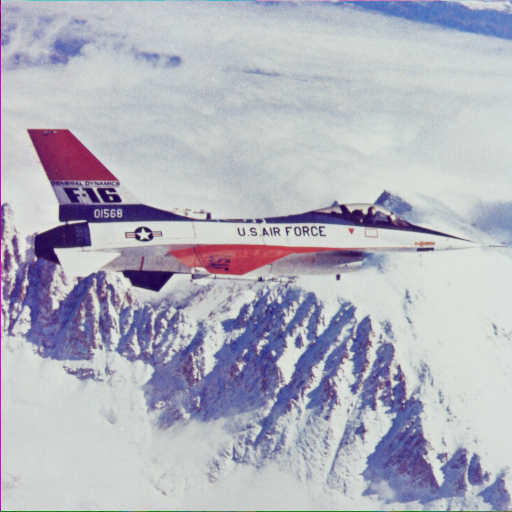
\includegraphics[width=5cm]{experiments/airplane}
                }
                \hspace{8pt}
                \subfloat[][Baboon (Mandrill)]{
                    \label{fig:exp-images-baboon}
                    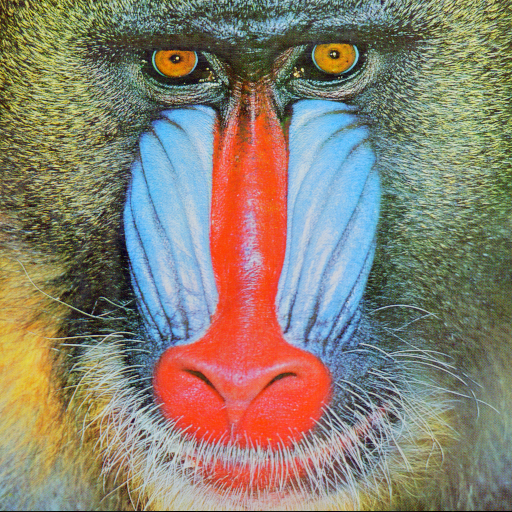
\includegraphics[width=5cm]{experiments/mandrill}
                } \\
                \subfloat[][House]{
                    \label{fig:exp-images-house}
                    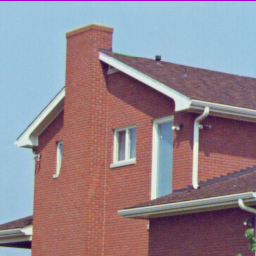
\includegraphics[width=5cm]{experiments/house}
                }
                \hspace{8pt}
                \subfloat[][Peppers]{
                    \label{fig:exp-images-peppers}
                    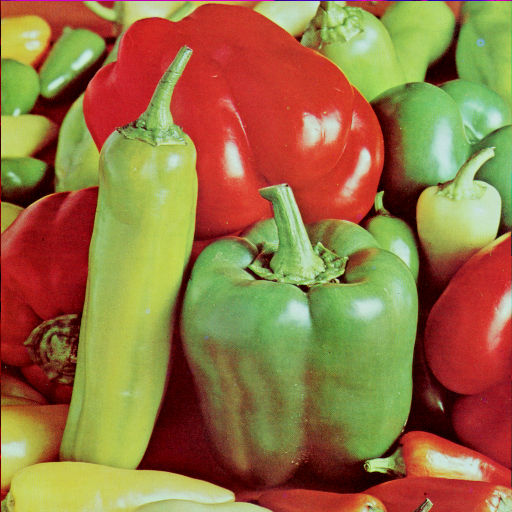
\includegraphics[width=5cm]{experiments/peppers}
                }

                \caption[Porównanie obrazów]
                {Obrazy wykorzystane w eksperymentach}
                \label{fig:exp-images}
            \end{figure}
        }

        % DANE
        \subsection{Dane}
        {
            %
            Dane które ukrywano w obrazach miały postać tekstu w formacie \textit{ASCII}, lecz po drobnych adaptacjach
            metody ukrywania danych w obrazie możliwe byłoby ukrywanie dowolnych danych w postaci binarnej. W
            eksperymentach wykorzystano automatycznie wygenerowany tekst \textit{Lorem ipsum} o rozmiarze $625kB$, lecz
            podczas eksperymentów wykorzystywano jedynie jego część. Cechą zaproponowanej metody oraz zaimplementowanego
            programu jest możliwość skalowania wygenerowanej macierzy maskującej w taki sposób, aby można było umieścić
            zadaną liczbę bitów tekstu. Pozwala to na zbadanie degradacji jakości w zależności od objętości ukrywanego
            tekstu oraz ułatwi porównanie rezultatów z innymi metodami.
            %
        }

        % BADANE PARAMETRY
        \subsection{Badane parametry}
        {
            Podczas przeprowadzanych eksperymentów badano wykorzystane metody każdego z etapów procesu oraz ich
            parametry. Porównywane wartości parametrów dotyczą:

            \begin{enumerate}
                \item Konstrukcji grafu oraz wizualizacji śladu feromonowego.
                \begin{itemize}
                    \item Metoda oparta na wierzchołkach. Jedynym parametrem jest opcjonalny parametr $s_0$ skalujący
                    obraz wejściowy podczas budowania grafu oraz budowania macierzy maskującej. Jego wartości znajdują
                    się w zakresie $[0, 1]$. Jego domyślna wartość wynosi $1$ i oznacza budowanie grafu o liczbie
                    wierzchołków równej $w \cdot h$.

                    \item Metoda oparta na krawędziach. Do jej parametrów należy algorytm segmentacji oraz docelowa
                    liczba segmentów $N_s$ związana z liczbą krawędzi grafu. Podczas badań wykorzystano algorytmy
                    prostego podziału na prostokąty, algorytm \textit{k}-średnich oraz algorytm \textit{SLIC} służący do
                    konstrukcji superpikseli.
                \end{itemize}

                \item Wyznaczenie śladu feromonowego przez różne rodzaje systemów mrówkowych. Do parametrów wspólnych
                dla każdego z wykorzystanych systemów należą:
                \begin{itemize}
                    \item liczba mrówek $A$, która domyślnie jest równa liczbie wierzchołków grafu $V$,
                    \item liczba wykonanych cykli $C$,
                    \item liczba kroków wykonywanych przez mrówki w każdej iteracji algorytmu $S$, dla grafów
                    skonstruowanych na podstawie segmentacji obrazu jest ona równa liczbie wierzchołków $V$,
                    \item preferencja względem śladu feromonowego $\alpha$,
                    \item preferencja względem widoczności wierzchołka $\beta$,
                    \item początkowa wartość śladu feromonowego $\tau_0$,
                    \item współczynnik opisujący szybkość wyparowania śladu feromonowego $\rho$.
                \end{itemize}

                Do porównanych rodzajów systemów należą poniższe odmiany (z niektórymi z nich związane są dodatkowe
                parametry oraz domyślne wartości powyższych):
                \begin{itemize}
                    \item model: feromon stały,
                    \item model: feromon średni,
                    \item model: feromon cykliczny,
                    \item system mrowiskowy, który wprowadza prawdopodobieństwo eksploatacji $q_0$ oraz ustala parametr
                    $\alpha = 1$,
                    \item system max-min, który wprowadza ograniczenia wartości śladu feromonowego $[\tau_{min},
                    \tau_{max}]$. Ich wartości wyznaczane są za pomocą estymaty dotyczącej długości poszukiwanego cyklu.
                    Wartość początkowa feromonu wynosi $\tau_0 = \tau_{max}$.
                \end{itemize}
            \end{enumerate}
        }
    }

    % WYKORZYSTANE MIARY JAKOŚCI
    \section{Miary jakości}\label{sec:measures}
    {
        W celu umożliwienia porównywania jakości steganogramów, zdecydowano się skorzystać z metryk służących do
        porównawczej analizy obrazów. Zastosowane metryki można podzielić na dwie kategorie, obiektywne i subiektywne.
        Metryki obiektywne służą do wyznaczenia pewnej wartości charakteryzującej różnicę pomiędzy dwoma sygnałami. W
        przypadku metryk subiektywnych, ich zadaniem jest również wyznaczenie wartości numerycznej, lecz nacisk
        kładziony jest na korelację wartości z postrzegalnością zmian przez ludzki układ wzrokowy. Do zastosowanych
        metryk należą:

        \begin{itemize}
            \item Błąd średniokwadratowy (ang. \textit{Mean Square Error - MSE}).

            Jest jedną z najprostszych metryk służących do pomiaru różnic między obrazami. Jego wartości należą do
            zbioru nieujemnych liczb rzeczywistych, a wartości bliższe zeru stanowią o mniejszym spadku jakości. Do jej
            zalet należy prostota implementacji i możliwość optymalnej implementacji. Jedną z jej wad jest niska
            korelacja z postrzeganiem różnic między obrazami przez ludzi oraz nieuwzględnianie informacji o relacji
            natężenia szumu do wartości sygnału. Jego wartość wyraża wzór:

            \begin{equation}\label{eqt:mse}
                \mathit{MSE} = \frac{1}{n} \sum_{i=1}^n (X_i - \overline{X})
            \end{equation}

            gdzie:
            \begin{description}
                \item $n$ - ilość obserwacji
                \item $X_i$ - wartość sygnału
                \item $\overline{X}$ - średnia wartość sygnału
            \end{description}

            \item Szczytowy stosunek sygnału do szumu (ang. \textit{Peak Signal Noise Ratio - PSNR}).

            Jest udoskonaleniem błędu średniokwadratowego, gdyż metryka ta uzależnia swoją wartość od maksymalnej
            wartości przyjmowanej przez sygnał. Oznacza to, że taka sama wartość \textit{PSNR} odpowiada różnicom
            będących w proporcjonalnym do ilości informacji. Przykładowo, w przypadku \textit{MSE} ta sama wartość
            będzie przekładać się na różną postrzegalność błędu w obrazie korzystającym z 8 i 24 bitów na kanał.
            Szczytowy stosunek sygnału do szumu rozwiązuje powyższy problem. W związku z dużym zakresem przyjmowanych
            wartości metryka korzysta z skali logarytmicznej. Wartościami typowymi przy analizie obrazów korzystających
            z 8 bitów na jeden kanał jest zakres $[30dB, 50dB]$, przy czym wyższa wartość oznacza mniejszą degradację.
            Wartość metryki można wyznaczyć za pomocą wzoru:

            \begin{equation}\label{eqt:psnr}
                \mathit{PSNR} = 10 \cdot log_{10} \frac{\mathit{MAX}^2}{\mathit{MSE}}
            \end{equation}

            gdzie:
            \begin{description}
                \item $\mathit{MAX}$ - maksymalna wartość sygnału
                \item $\mathit{MSE}$ - błąd średniokwadratowy
            \end{description}

            \item Indeks podobieństwa strukturalnego (ang. \textit{Structural Similarity Index, SSIM}).

            Zdecydowanie bardziej złożoną metryką jest \textit{SSIM}. Jej celem jest uchwycenie złożoności i cech
            postrzegania ludzkiego systemu wzrokowego. Opiera się na założeniu mówiącym o istotności struktury obrazu w
            odniesieniu do postrzeganych różnic luminancji oraz kontrastu \cite{Wang2004ImageQA, Sara2019ImageQA}. Jej
            wartość jest zwykle normalizowana do zakresu $[0, 1]$, gdzie wartość $1$ oznacza identyczność obrazów.
        \end{itemize}
    }

    % WYNIKI EKSPERYMENTÓW
    \section{Wyniki eksperymentów}
    {
        %
        Eksperymenty rozpoczęto od analizy wyników uzyskanych metodą opartą na budowaniu grafu na podstawie
        wierzchołków.

        % WYNIKI - METODA-WIERZCHOŁKÓW - INVERTED
        \subsection{Metoda oparta na wierzchołkach}
        {
            Eksperymenty rozpoczęto od porównania wpływu proporcjonalności długości krawędzi grafu do różnicy pomiędzy
            pikselami. Jak wspomniano w rozdziale \ref{sec:method}, jeśli długości krawędzi są proporcjonalne do różnicy
            pikseli, system mrówkowy będzie dążył do odkładania śladu feromonowego w obszarach cechujących mniejszą
            złożoność. Aby uzyskać zamierzony rezultat, czyli macierz maskującą wskazującą obszary bardziej złożone,
            konieczne jest odwrócenie jej wartości. Alternatywnie, jeśli długości pomiędzy pikselami będą odwrotnie
            proporcjonalne do dzielącej je odległości, system mrówkowy, a co za tym idzie ślad feromonowy, będzie
            preferował obszary bardziej złożone.

            Wizualizację procesu konwersji obrazu na graf oraz uzyskane macierze maskujące przedstawia rysunek
            \ref{fig:exp-vertex}. W pierwszej kolumnie umieszczono obrazy objaśniające wynik konwersji bitmapy na graf,
            w których do poszczególnych pikseli obrazu wejściowego przypisana jest luminancja odwrotnie proporcjonalna
            do długości krawędzi z nim związanych (obszary ,,atrakcyjniejsze'' dla mrówek cechują się są reprezentowane
            przez jaśniejsze piksele). Kolumna druga przedstawia macierze maskujące, które będą decydować o liczbie
            bitów, które zostaną zamienione na bity ukrywanej wiadomości. Im jaśniejszy jest dany piksel, tym więcej
            jego bitów zostanie zamienionych. W trzeciej kolumnie przedstawiono macierze maskujące przetransformowane w
            taki sposób, aby odpowiadające im pojemność ukrywanej wiadomości była taka sama.

            Na podstawie obrazów \ref{fig:exp-vertex-pher} oraz \ref{fig:exp-vertex-inv-pher} można stwierdzić, że obie
            metody poprawnie wykrywają krawędzie i obszary złożone, lecz po porównaniu macierzy maskujących o tej samej
            pojemności należy stwierdzić lepszy rezultat procesu, w którym długości krawędzi grafu są proporcjonalne do
            różnicy pomiędzy pikselami, a macierz maskująca zostaje odwrócona. Przeskalowana macierz maskująca
            \ref{fig:exp-vertex-inv-pher-scaled} gwarantuje bardziej równomierne rozłożenie informacji przy jednoczesnym
            faworyzowaniu obszarów złożonych.

            \begin{figure}
                \centering
                \subfloat[][]{
                    \label{fig:exp-vertex-conv}
                    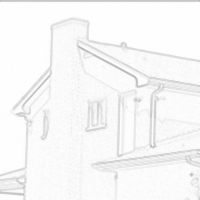
\includegraphics[width=4cm]{experiments/vertexbased/normal-vs-inverted/2021-04-17-06:25:53house-l_conv_a1000_s100_Dbasic:_Uconst:_Cspatial:_c10_m0_t50000B_}

                }
                \hspace{8pt}
                \subfloat[][]{
                    \label{fig:exp-vertex-pher}
                    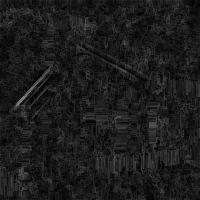
\includegraphics[width=4cm]{experiments/vertexbased/normal-vs-inverted/2021-04-17-06:25:53house-l_pher_a1000_s100_Dbasic:_Uconst:_Cspatial:_c10_m0_t50000B_}
                }
                \hspace{8pt}
                \subfloat[][]{
                    \label{fig:exp-vertex-pher-scaled}
                    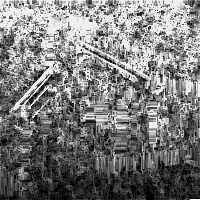
\includegraphics[width=4cm]{experiments/vertexbased/normal-vs-inverted/2021-04-17-06:25:53house-l_pher_scaled_a1000_s100_Dbasic:_Uconst:_Cspatial:_c10_m0_t50000B_}
                } \\
                \subfloat[][]{
                    \label{fig:exp-vertex-inv-conv}
                    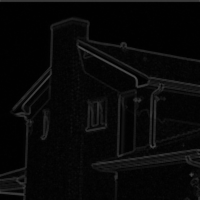
\includegraphics[width=4cm]{experiments/vertexbased/normal-vs-inverted/2021-04-17-06:26:02house-l_conv_a1000_s100_Dbasic:_Uconst:_Ci:spatial:_c10_m0_t50000B_}
                }
                \hspace{8pt}
                \subfloat[][]{
                    \label{fig:exp-vertex-inv-pher}
                    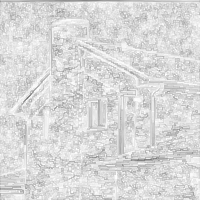
\includegraphics[width=4cm]{experiments/vertexbased/normal-vs-inverted/2021-04-17-06:26:02house-l_pher_a1000_s100_Dbasic:_Uconst:_Ci:spatial:_c10_m0_t50000B_}
                } \subfloat[][]{
                    \label{fig:exp-vertex-inv-pher-scaled}
                    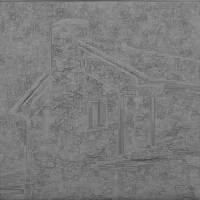
\includegraphics[width=4cm]{experiments/vertexbased/normal-vs-inverted/2021-04-17-06:26:02house-l_pher_scaled_a1000_s100_Dbasic:_Uconst:_Ci:spatial:_c10_m0_t50000B_}
                }

                \caption[Porównania wizualizacji konwersji oraz macierzy maskujących.]
                {Porównania wizualizacji konwersji oraz macierzy maskujących. W pierwszym wierszu
                    (\subref{fig:exp-vertex-conv}, \subref{fig:exp-vertex-pher}, \subref{fig:exp-vertex-pher-scaled})
                    przedstawiono obrazy związane z procesem o długości krawędzi odwrotnie proporcjonalnej do różnicy
                    pikseli. W drugim wierszu (\subref{fig:exp-vertex-inv-conv}, \subref{fig:exp-vertex-inv-pher},
                    \subref{fig:exp-vertex-inv-pher-scaled}) długości są proporcjonalne do różnicy pikseli. Pierwsza
                    kolumna przedstawia wizualizacje procesu konwersji bitmapy na graf, druga przestawia uzyskane
                    macierze maskujące, trzecia zawiera macierze maskujące przeskalowane w taki sposób, aby odpowiadała
                    im taka sama pojemność ukrywanej informacji}
                \label{fig:exp-vertex}
            \end{figure}

            % WYNIKI - METODA-WIERZCHOŁKÓW - RODZAJE SYSTEMÓW
            Kolejnym parametrem, który postanowiono zbadać, jest rodzaj systemu mrówkowego oraz związane z nim
            parametry. Ponieważ problem rozwiązywany przez mrówki nie jest równoważny z problemem komiwojażera,
            konieczne jest również ustalenie parametru $S$ określającego liczbę kroków wykonywanych przez każdą mrówkę w
            każdej iteracji algorytmu.

            Wygenerowane macierze maskujące przedstawia rysunek \ref{fig:exp-vertex-pher}. Na ich podstawie można
            wyciągnąć kilka interesujących wniosków. System mrowiskowy (\textit{Ant-Colony}) oraz system
            \textit{Max-min} nie odpowiadają charakterystyce zadanego zadania, które jest znacząco różne od klasycznego
            problemu \textit{TSP}. Przyczyn można doszukiwać się w silnej faworyzacji najlepszego rozwiązania, czyli
            najkrótszej obranej ścieżki kosztem pozostałych ścieżek. Można wnioskować, że w przedstawionym problemie
            znalezienie najkrótszej ścieżki łączącej $S + 1$ pikseli spośród pikseli obrazu o wymiarach $w \times h$ nie
            przyczynia się do ogólnego wyznaczenia obszarów obrazu.

            Na dodatkową uwagę zasługuje system z cykliczną regułą aktualizacji śladu feromonowego, gdyż za jego pomocą
            udało się wyraźnie wyodrębnić jednorodny obszar nieba oraz pewne homogeniczne elementy budynku. Kolejną
            obserwacją płynącą z powyższego eksperymentu jest istotność doboru liczby mrówek $A$ oraz współczynnika
            związanego z odparowaniem śladu $\rho$. Macierze lepiej odzwierciedlające faktyczne segmenty obrazów
            powstały w przypadku konfiguracji charakteryzujących się większą liczbą mrówek (na przykład
            \ref{fig:exp-vertex-pher-pher-cycle3}) lub wyższym współczynnikiem $\rho$ (na przykład
            \ref{fig:exp-vertex-pher-conv-const1}), przekładającym się na wolniejsze tempo odparowania.

            \begin{figure}
                \footnotesize
                \centering
                \subfloat[][Ant-Density\newline $A=1000$, $S=100$ \newline $\alpha=2$, $\beta=1$, $\rho=0.8$]{
                    \label{fig:exp-vertex-pher-conv-const1}
                    
\includegraphics[width=3cm]{experiments/vertexbased/colony-types/2021-04-17-12:29:22house-l_pher_a1000_s100_Dbiased:2,1_Uconst:1,0.2,1_Ci:spatial:_c10_m0_t100000B_}
                }
                \hspace{8pt}
                \subfloat[][Ant-Density\newline $A=1000$, $S=100$ \newline $\alpha=2$, $\beta=2$, $\rho=0.9$]{
                    \label{fig:exp-vertex-pher-pher-const2}
                    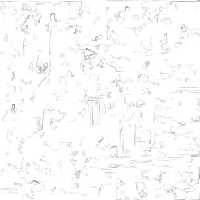
\includegraphics[width=3cm]{experiments/vertexbased/colony-types/2021-04-17-12:29:25house-l_pher_a1000_s100_Dbiased:2,2_Uconst:1,0.1,1_Ci:spatial:_c10_m0_t100000B_}
                }
                \hspace{8pt}
                \subfloat[][Ant-Density\newline $A=1000$, $S=100$ \newline $\alpha=2$, $\beta=2$, $\rho=0.999$]{
                    \label{fig:exp-vertex-pher-pher-const3}
                    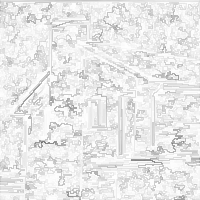
\includegraphics[width=3cm]{experiments/vertexbased/colony-types/2021-04-17-12:29:25house-l_pher_a1000_s100_Dbiased:2,2_Uconst:1,0.001,1_Ci:spatial:_c10_m0_t100000B_}
                } \\
                \subfloat[][Ant-Quantity\newline $A=1000$, $S=100$ \newline $\alpha=1$, $\beta=1$, $\rho=0.8$]{
                    \label{fig:exp-vertex-pher-pher-avg1}
                    
\includegraphics[width=3cm]{experiments/vertexbased/colony-types/2021-04-17-12:29:31house-l_pher_a1000_s100_Dbiased:1,1_Uavg:1,0.2,1_Ci:spatial:_c10_m0_t100000B_}
                }
                \hspace{8pt}
                \subfloat[][Ant-Quantity\newline $A=1000$, $S=100$ \newline $\alpha=2$, $\beta=2$, $\rho=0.999$]{
                    \label{fig:exp-vertex-pher-pher-avg2}
                    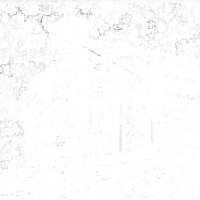
\includegraphics[width=3cm]{experiments/vertexbased/colony-types/2021-04-17-12:29:29house-l_pher_a1000_s100_Dbiased:2,2_Uavg:1,0.001,1_Ci:spatial:_c10_m0_t100000B_}
                } \subfloat[][Ant-Quantity\newline $A=10000$, $S=10$ \newline $\alpha=1$, $\beta=1$, $\rho=0.8$]{
                    \label{fig:exp-vertex-pher-pher-avg3}
                    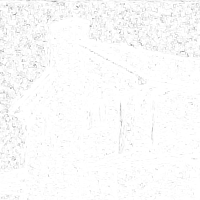
\includegraphics[width=3cm]{experiments/vertexbased/colony-types/2021-04-17-12:29:12house-l_pher_a10000_s10_Dbiased:1,1_Uavg:1,0.2,1_Ci:spatial:_c10_m0_t100000B_}
                } \\
                \subfloat[][Ant-Cycle\newline $A=10$, $S=10000$ \newline $\alpha=1$, $\beta=1$, $\rho=0.8$]{
                    \label{fig:exp-vertex-pher-pher-cycle1}
                    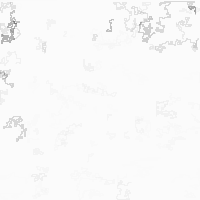
\includegraphics[width=3cm]{experiments/vertexbased/colony-types/2021-04-17-12:29:38house-l_pher_a10_s10000_Dbiased:1,1_Ucycle:1,0.2,1,10000_Ci:spatial:_c10_m0_t100000B_}
                }
                \hspace{8pt}
                \subfloat[][Ant-Cycle\newline $A=1000$, $S=100$ \newline $\alpha=1$, $\beta=1$, $\rho=0.8$]{
                    \label{fig:exp-vertex-pher-pher-cycle2}
                    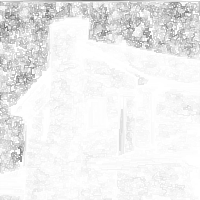
\includegraphics[width=3cm]{experiments/vertexbased/colony-types/2021-04-17-12:29:26house-l_pher_a1000_s100_Dbiased:1,1_Ucycle:1,0.2,1,100_Ci:spatial:_c10_m0_t100000B_}
                } \subfloat[][Ant-Cycle\newline $A=10000$, $S=10$ \newline $\alpha=1$, $\beta=1$, $\rho=0.8$]{

                    \label{fig:exp-vertex-pher-pher-cycle3}
                    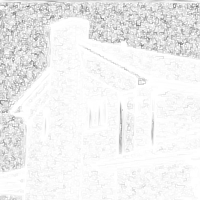
\includegraphics[width=3cm]{experiments/vertexbased/colony-types/2021-04-17-12:29:10house-l_pher_a10000_s10_Dbiased:1,1_Ucycle:1,0.2,1,10_Ci:spatial:_c10_m0_t100000B_}
                } \\
                \subfloat[][Ant-Colony\newline $A=10$, $S=10000$ \newline $\alpha=1$, $\beta=1$, $\rho=0.999$]{
                    \label{fig:exp-vertex-pher-pher-colony1}
                    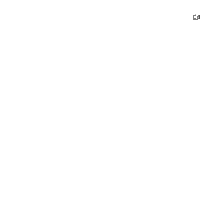
\includegraphics[width=3cm]{experiments/vertexbased/colony-types/2021-04-17-12:35:20house-l_pher_a10_s10000_Dcolony:0.1,1_Ucolony:1,0.2,0.2,10000_Ci:spatial:_c10_m0_t100000B_}
                }
                \hspace{8pt}
                \subfloat[][Ant-Colony\newline $A=1000$, $S=100$ \newline $\alpha=1$, $\beta=2$, $\rho=0.999$]{
                    \label{fig:exp-vertex-pher-pher-colony2}
                    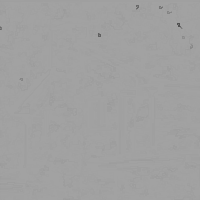
\includegraphics[width=3cm]{experiments/vertexbased/colony-types/2021-04-17-12:29:29house-l_pher_a1000_s100_Dcolony:0.1,2_Ucolony:1,0.001,0.001,100_Ci:spatial:_c10_m0_t100000B_}
                } \subfloat[][Ant-Colony\newline $A=10000$, $S=10$ \newline $\alpha=1$, $\beta=1$, $\rho=0.8$]{
                    \label{fig:exp-vertex-pher-pher-colony3}
                    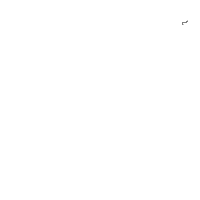
\includegraphics[width=3cm]{experiments/vertexbased/colony-types/2021-04-17-12:29:11house-l_pher_a10000_s10_Dcolony:0.1,1_Ucolony:1,0.2,0.2,10_Ci:spatial:_c10_m0_t100000B_}
                } \\
                \subfloat[][Max-Min\newline $A=10$, $S=10000$ \newline $\alpha=1$, $\beta=1$, $\rho=0.8$]{
                    \label{fig:exp-vertex-pher-pher-maxmin1}
                    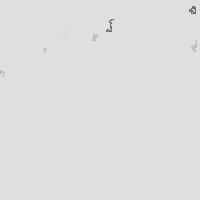
\includegraphics[width=3cm]{experiments/vertexbased/colony-types/2021-04-17-12:29:38house-l_pher_a10_s10000_Dbiased:1,1_Umaxmin:1,0.2,0.1,10000_Ci:spatial:_c10_m0_t100000B_}
                }
                \hspace{8pt}
                \subfloat[][Max-Min\newline $A=1000$, $S=100$ \newline $\alpha=2$, $\beta=2$, $\rho=0.999$]{
                    \label{fig:exp-vertex-pher-pher-maxmin2}
                    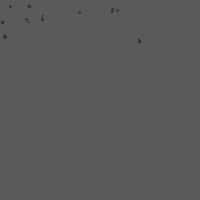
\includegraphics[width=3cm]{experiments/vertexbased/colony-types/2021-04-17-12:29:27house-l_pher_a1000_s100_Dbiased:2,2_Umaxmin:1,0.001,0.1,100_Ci:spatial:_c10_m0_t100000B_}
                } \subfloat[][Max-Min\newline $A=10000$, $S=10$ \newline $\alpha=1$, $\beta=1$, $\rho=0.9$]{
                    \label{fig:exp-vertex-pher-pher-maxmin3}
                    
\includegraphics[width=3cm]{experiments/vertexbased/colony-types/2021-04-17-12:29:12house-l_pher_a10000_s10_Dbiased:1,1_Umaxmin:1,0.2,0.1,10_Ci:spatial:_c10_m0_t100000B_}
                }

                \caption[Porównania wizualizacji konwersji oraz macierzy maskujących.]
                {Macierze maskujące wygenerowane za pomocą różnych systemów mrówkowych}
                \label{fig:exp-vertex-pher}
            \end{figure}

            % METODA WIERZCHOŁKÓW - SKALOWANIE OBRAZU
            Ponieważ pozostałe obrazy z zbioru \textit{USC} mają rozmiary $512 \times 512$, zdecydowano się również
            zbadać wpływ skalowania obrazu podczas tworzenia grafu oraz macierzy maskującej. Wykorzystano system oparty
            na modelu cyklicznym o parametrach $A=10000$, $S=100$, $\alpha=\beta=1$, $\rho=0.8$, i starano się umieścić
            $250kB$ danych. Na rysunku \ref{fig:exp-vertex-scale} zamieszczono macierze maskujące powstałe przy $s_0 \in
            \{0.25, 0.5, 0.75, 1.0\}$. Tabela \ref{tab:exp-vertex-scale-errors} zawiera porównanie miar jakości
            steganogramów.

            Na postawie uzyskanych wyników można stwierdzić że tworzenie grafu na podstawie skalowanego obrazu nie ma
            znaczącego wpływu na miary jakości steganogramu. Jest to pożądana cecha, ponieważ operacje na mniejszych
            grafach zajmują zdecydowanie mniej czasu.

            \begin{figure}
                \footnotesize
                \centering
                \subfloat[][Macierz maskująca\newline $s_0 = 0.25$]{
                    \label{fig:exp-vertex-scale0.25-pher}
                    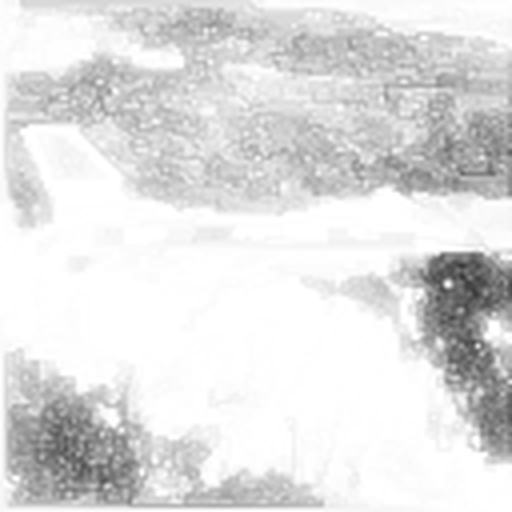
\includegraphics[width=4cm]{experiments/vertexbased/scaling/2021-04-17-15:53:35airplane_pher_a10000_s100_Dbiased:1,1_Ucycle:1,0.2,1,100_Ci:spatial:_c10_m128_t250000B_}
                }
                \hspace{8pt}
                \subfloat[][Steganogram\newline $s_0 = 0.25$]{
                    \label{fig:exp-vertex-scale0.25-steg}
                    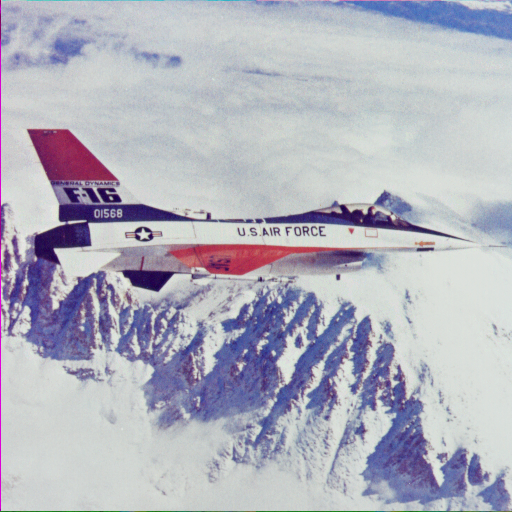
\includegraphics[width=4cm]{experiments/vertexbased/scaling/2021-04-17-15:53:35airplane_steg_a10000_s100_Dbiased:1,1_Ucycle:1,0.2,1,100_Ci:spatial:_c10_m128_t250000B_}
                } \\
                \subfloat[][Macierz maskująca\newline $s_0 = 0.5$]{
                    \label{fig:exp-vertex-scale0.50-pher}
                    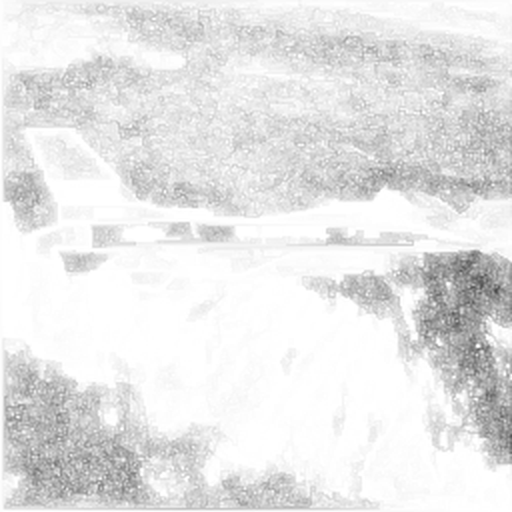
\includegraphics[width=4cm]{experiments/vertexbased/scaling/2021-04-17-15:53:51airplane_pher_a10000_s100_Dbiased:1,1_Ucycle:1,0.2,1,100_Ci:spatial:_c10_m256_t250000B_}
                }
                \hspace{8pt}
                \subfloat[][Steganogram\newline $s_0 = 0.5$]{
                    \label{fig:exp-vertex-scale0.50-steg}
                    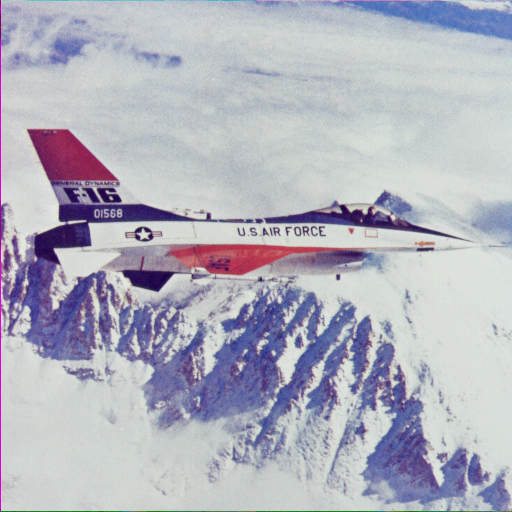
\includegraphics[width=4cm]{experiments/vertexbased/scaling/2021-04-17-15:53:51airplane_steg_a10000_s100_Dbiased:1,1_Ucycle:1,0.2,1,100_Ci:spatial:_c10_m256_t250000B_}
                } \\
                \subfloat[][Macierz maskująca\newline $s_0 = 0.75$]{
                    \label{fig:exp-vertex-scale0.75-pher}
                    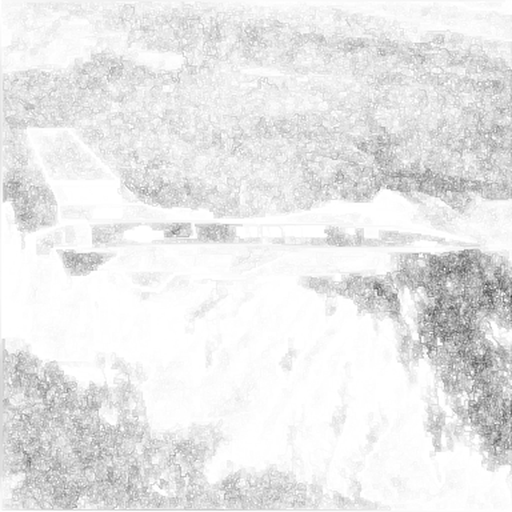
\includegraphics[width=4cm]{experiments/vertexbased/scaling/2021-04-17-15:56:42airplane_pher_a10000_s100_Dbiased:1,1_Ucycle:1,0.2,1,100_Ci:spatial:_c10_m384_t250000B_}
                }
                \hspace{8pt}
                \subfloat[][Steganogram\newline $s_0 = 0.75$]{

                    \label{fig:exp-vertex-scale0.75-steg}
                    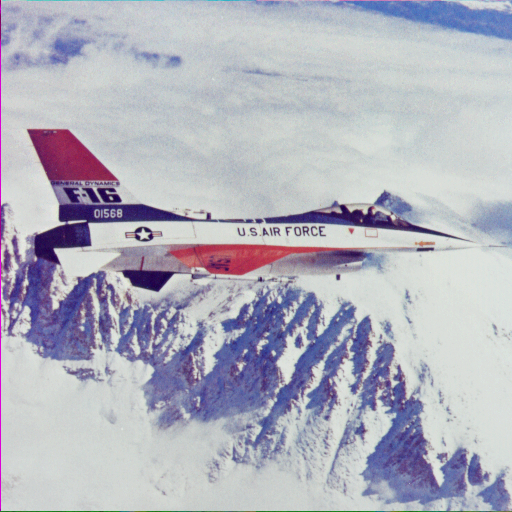
\includegraphics[width=4cm]{experiments/vertexbased/scaling/2021-04-17-15:56:43airplane_steg_a10000_s100_Dbiased:1,1_Ucycle:1,0.2,1,100_Ci:spatial:_c10_m384_t250000B_}
                } \\
                \subfloat[][Macierz maskująca\newline $s_0 = 1.0$]{
                    \label{fig:exp-vertex-scale1.0-pher}
                    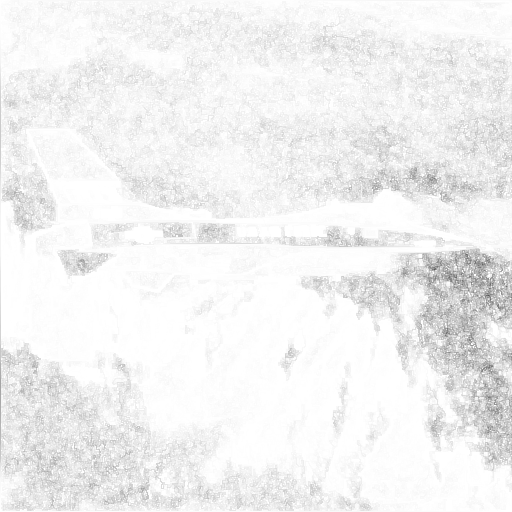
\includegraphics[width=4cm]{experiments/vertexbased/scaling/2021-04-17-15:54:02airplane_pher_a10000_s100_Dbiased:1,1_Ucycle:1,0.2,1,100_Ci:spatial:_c10_m0_t250000B_}
                }
                \hspace{8pt}
                \subfloat[][Steganogram\newline $s_0 = 1.0$]{
                    \label{fig:exp-vertex-scale1.0-steg}
                    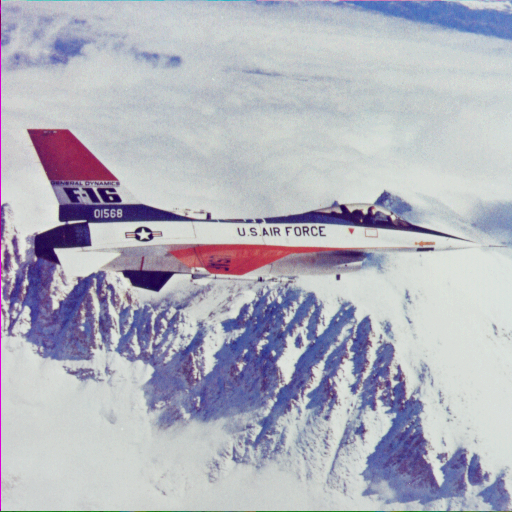
\includegraphics[width=4cm]{experiments/vertexbased/scaling/2021-04-17-15:54:02airplane_steg_a10000_s100_Dbiased:1,1_Ucycle:1,0.2,1,100_Ci:spatial:_c10_m0_t250000B_}
                }

                \caption[Porównania wizualizacji konwersji oraz macierzy maskujących.]
                {Macierze maskujące oraz steganogramy wygenerowane dla różnych wartości skali $s_0$}
                \label{fig:exp-vertex-scale}
            \end{figure}

            \begin{table}
                \centering
                \caption{Miary jakości steganogramów w zależności od współczynnika $s_0$. W tabeli pogrubiono wartości poszczególnych miar wskazujące na najniższy spadek jakości}
                \begin{tabular}{ |c|c c c| }
                    \hline
                    Współczynnik skalujący \newline $s_0$ & $MSE$ & $PSNR$ & $SSIM$ \\
                    \hline
                    0.25 & 6.93092 & 39.7568dB & \textbf{0.952935} \\
                    0.5 & 6.67252 & 39.9218dB & 0.951723 \\
                    0.75 & 6.62924 & 39.9501dB & 0.95122 \\
                    1.0 & \textbf{6.61124} & \textbf{39.9619dB} & 0.948736 \\
                    \hline
                \end{tabular}
                \label{tab:exp-vertex-scale-errors}
            \end{table}

            % METODA WIERZCHOŁKÓW - FINAL SHOWDOWN
            Ostatecznie, postanowiono zbadać wyniki uzyskane na pozostałych obrazach testowych. Uzyskane rezultaty
            zawiera tabela \ref{tab:exp-vertex-results}, a steganogramy rysunek \ref{fig:exp-vertex-results}. Parametry
            algorytmu zachowano z poprzedniego eksperymentu.

            \begin{table}
                \centering
                \caption{Wyniki uzyskane metodą opartą na wierzchołkach}
                \begin{tabular}{ |l|c|c c c| }
                    \hline
                    Obraz & objętość danych & $MSE$ & $PSNR$ & $SSIM$ \\
                    \hline
                    Baboon {\footnotesize $512 \times 512$}   & 100 000B (12.71\%) & 0.538851 & 50.85dB & 0.998768 \\
                    Baboon {\footnotesize $512 \times 512$}   & 250 000B (31.78\%) & 6.60594 & 39.9654dB & 0.990015 \\
                    Baboon {\footnotesize $512 \times 512$}   & 500 000B (63.57\%) & 272.732 & 23.8074dB & 0.777025 \\
                    Airplane {\footnotesize $512 \times 512$} & 100 000B (12.71\%) & 0.53689 & 50.8659dB & 0.995503 \\
                    Airplane {\footnotesize $512 \times 512$} & 250 000B (31.78\%) & 6.67252 & 39.9218dB & 0.951723 \\
                    Airplane {\footnotesize $512 \times 512$} & 500 000B (63.57\%) & 311.43 & 23.2311dB & 0.516503 \\
                    Peppers {\footnotesize $512 \times 512$}  & 100 000B (12.71\%) & 0.536934 & 50.8655dB & 0.996048 \\
                    Peppers {\footnotesize $512 \times 512$}  & 250 000B (31.78\%) & 6.71828 & 39.8922dB & 0.958181 \\
                    Peppers {\footnotesize $512 \times 512$}  & 500 000B (63.57\%) & 292.99 & 23.4962dB & 0.502009 \\
                    \hline
                \end{tabular}
                \label{tab:exp-vertex-results}
            \end{table}

            \begin{figure}
                \footnotesize
                \centering
                \subfloat[][$D = 100 000B$]{
                    \label{fig:exp-vertex-results-baboon-100k}
                    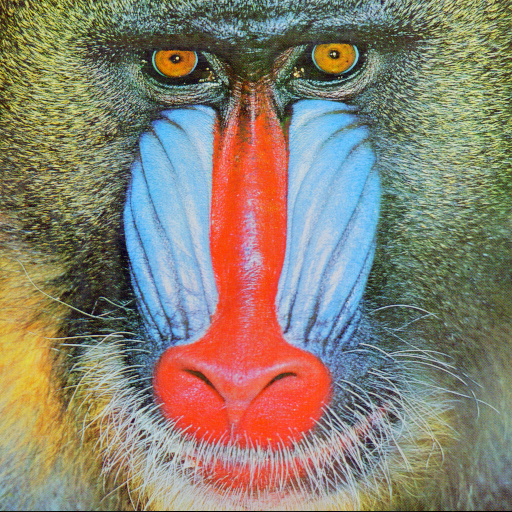
\includegraphics[width=3cm]{experiments/vertexbased/results/2021-04-17-17:12:31mandrill_steg_a10000_s100_Dbiased:1,1_Ucycle:1,0.2,1,100_Ci:spatial:_c10_m256_t100000B_}
                }
                \hspace{8pt}
                \subfloat[][$D = 250 000B$]{
                    \label{fig:exp-vertex-results-baboon-250k}
                    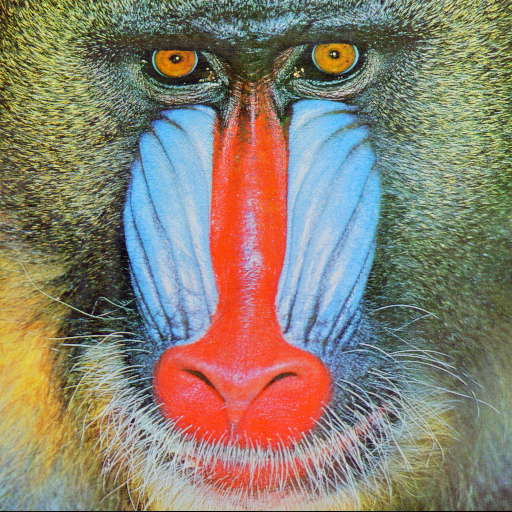
\includegraphics[width=3cm]{experiments/vertexbased/results/2021-04-17-17:13:06mandrill_steg_a10000_s100_Dbiased:1,1_Ucycle:1,0.2,1,100_Ci:spatial:_c10_m256_t250000B_}
                } \subfloat[][$D = 500 000B$]{
                    \label{fig:exp-vertex-results-baboon-500k}
                    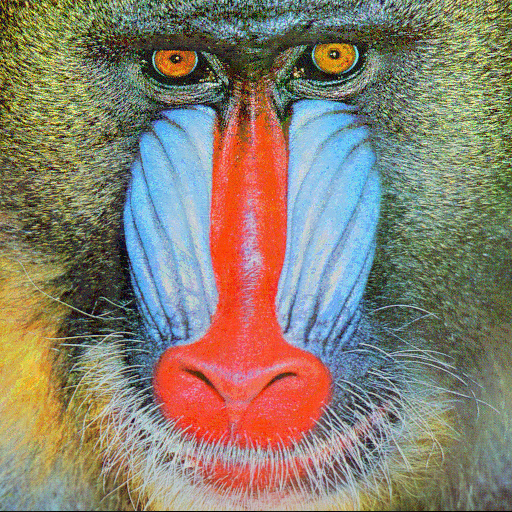
\includegraphics[width=3cm]{experiments/vertexbased/results/2021-04-17-17:13:33mandrill_steg_a10000_s100_Dbiased:1,1_Ucycle:1,0.2,1,100_Ci:spatial:_c10_m256_t500000B_}
                } \\
                \subfloat[][$D = 100 000B$]{
                    \label{fig:exp-vertex-results-aiplane-100k}
                    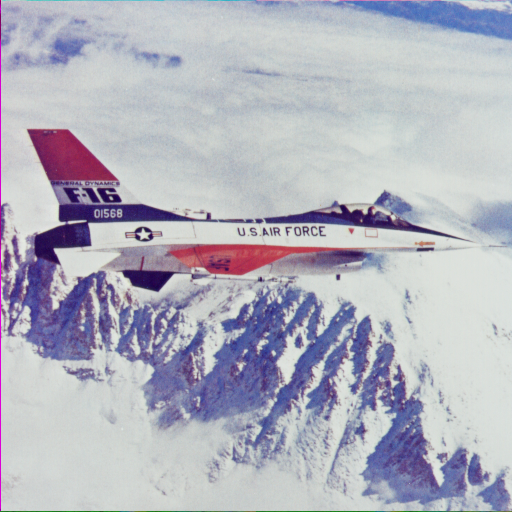
\includegraphics[width=3cm]{experiments/vertexbased/results/2021-04-17-17:16:39airplane_steg_a10000_s100_Dbiased:1,1_Ucycle:1,0.2,1,100_Ci:spatial:_c10_m256_t100000B_}
                }
                \hspace{8pt}
                \subfloat[][$D = 250 000B$]{
                    \label{fig:exp-vertex-results-aiplane-250k}
                    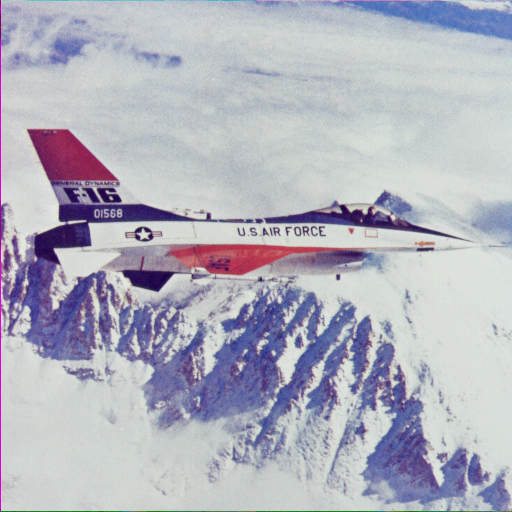
\includegraphics[width=3cm]{experiments/vertexbased/results/2021-04-17-17:17:10airplane_steg_a10000_s100_Dbiased:1,1_Ucycle:1,0.2,1,100_Ci:spatial:_c10_m256_t250000B_}
                }
                \hspace{8pt}
                \subfloat[][$D = 500 000B$]{
                    \label{fig:exp-vertex-results-aiplane-500k}
                    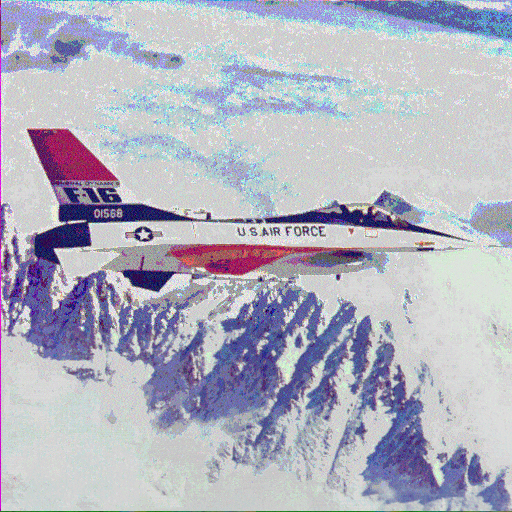
\includegraphics[width=3cm]{experiments/vertexbased/results/2021-04-17-17:17:35airplane_steg_a10000_s100_Dbiased:1,1_Ucycle:1,0.2,1,100_Ci:spatial:_c10_m256_t500000B_}
                } \\
                \subfloat[][$D = 100 000B$]{
                    \label{fig:exp-vertex-results-airplane-100k}
                    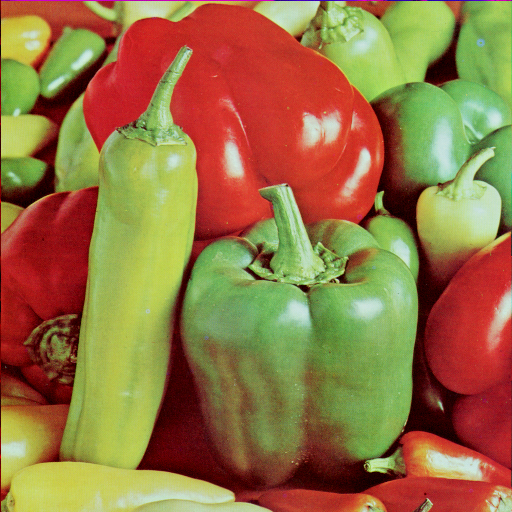
\includegraphics[width=3cm]{experiments/vertexbased/results/2021-04-17-17:18:34peppers_steg_a10000_s100_Dbiased:1,1_Ucycle:1,0.2,1,100_Ci:spatial:_c10_m256_t100000B_}
                }
                \hspace{8pt}
                \subfloat[][$D = 250 000B$]{
                    \label{fig:exp-vertex-results-airplane-250k}
                    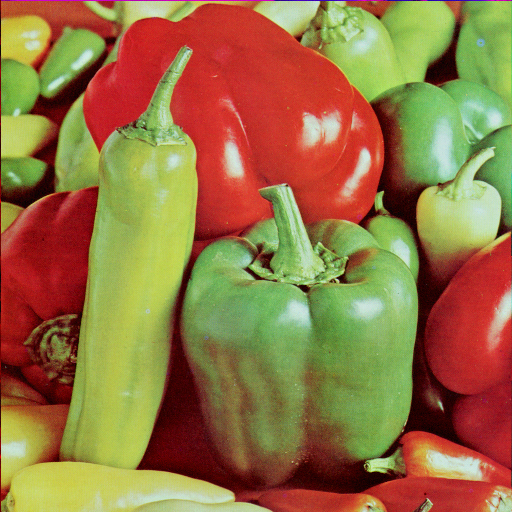
\includegraphics[width=3cm]{experiments/vertexbased/results/2021-04-17-17:19:05peppers_steg_a10000_s100_Dbiased:1,1_Ucycle:1,0.2,1,100_Ci:spatial:_c10_m256_t250000B_}
                } \subfloat[][$D = 500 000B$]{
                    \label{fig:exp-vertex-results-airplane-500k}
                    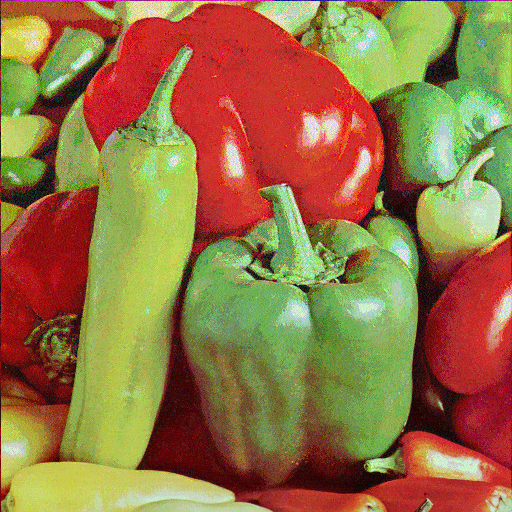
\includegraphics[width=3cm]{experiments/vertexbased/results/2021-04-17-17:19:31peppers_steg_a10000_s100_Dbiased:1,1_Ucycle:1,0.2,1,100_Ci:spatial:_c10_m256_t500000B_}
                }

                \caption[Porównanie rezultatów]
                {Porównanie uzyskanych steganogramów przy zadanej objętości ukrytej informacji}
                \label{fig:exp-vertex-results}
            \end{figure}
        }

        % WYNIKI - METODA-KRAWĘDZI
        \subsection{Metoda oparta na krawędziach}
        {
            Następnym krokiem eksperymentów było zbadanie metod opartych na budowanie grafu z wyznaczonych krawędzi. W
            przypadku tej metody, obraz jest dzielony na zadaną liczbę segmentów, które odpowiadają krawędziom
            tworzonego grafu pełnego. W związku z koniecznością budowy grafu pełnego, istotnym ograniczeniem metody jest
            konieczność takiego doboru liczby segmentów, aby spełniała one równanie wyrażające liczbę krawędzi $|E|$ w
            grafie pełnym o $|V|$ wierzchołkach $|E| = \frac{|V| \cdot (|V| - 1)}{2}$. Problem komiwojażera osadzony na
            tak utworzonym grafie można interpretować jako problem znalezienia $n$ segmentów obrazu tworzących
            najkrótszy cykl. Długości krawędzi tak powstałego grafu są zależne od różnicy wariancji łączących przez nie
            segmenty.

            % WYNIKI - METODA-KRAWĘDZI - INVERTED
            Podobnie jak w przypadku metody opisanej w sekcji powyżej, długości krawędzi grafu mogą być proporcjonalne
            lub odwrotnie proporcjonalne do wyznaczonej miary odległości. Z tego względu, postanowiono rozpatrzyć ten
            parametr jako pierwszy.

            Rysunek \ref{fig:exp-edge} przedstawia wizualizację utworzonego grafu oraz uzyskane ślady feromonowe.
            Porównywane obrazy zostały podzielone metodą superpikseli na $190$ segmentów ($|V| = 20$). Na podstawie
            uzyskanych steganogramów można łatwo zauważyć mankament wariantu, w którym długość krawędzi grafu jest
            odwrotnie proporcjonalna do różnicy wariancji segmentów (obrazy \ref{fig:exp-edge-conv},
            \ref{fig:exp-edge-pher}, \ref{fig:exp-edge-steg}).

            W przypadku rozwiązywania problemu \textit{TSP} ostatecznym wynikiem jest wybranie jedynie $|V|$ spośród
            wszystkich krawędzi, których jest $\frac{|V| \cdot (|V| - 1)}{2}$. Oznacza to, że gdy system mrówkowy
            osiągnie zbieżność ślad feromonowy na wszystkich krawędziach, poza należącymi do najkrótszej ścieżki, będzie
            bliski zeru. W takim przypadku, do ukrycia zadanej informacji zostanie wykorzystana jedynie znikoma część
            obrazu nośnego, co negatywnie wpływa na pojemność steganogramu. Wykres z rysunku \ref{fig:exp-edge-v-vs-e}
            przedstawia stosunek liczby $|V|$ do liczby krawędzi grafu w zależności od liczby jego wierzchołków.

            Powyższy problem można rozwiązać na co najmniej dwa sposoby. Pierwszym jest odpowiedni dobór parametrów
            systemu mrówkowego, który będzie wymuszał na mrówkach częstszą eksplorację (na przykład wybór dużej wartości
            $q_0$) lub częstszy wybór ścieżek w zachłanny sposób (przez dobór parametru $\alpha$). Dzięki temu, większa
            liczba krawędzi będzie odwiedzana, lecz wnosi to również ryzyko otrzymywania nieoptymalnych cykli.
            Alternatywą jest odwrócenie problemu reprezentowanego przez graf. Jeśli długości krawędzi będą
            proporcjonalne do różnic wariancji łączonych segmentów, mrówki będą dążyć do znalezienia $V$ krawędzi, w
            których nie należy umieszczać informacji, gdyż nie są wystarczająco złożone. W ten sposób, uzyskany ślad
            feromonowy wskaże $|V| - \frac{|V| \cdot (|V| - 1)}{2}$ segmentów, w których powinno zostać ukryte najwięcej
            informacji.

            \begin{figure}
                \centering
                \subfloat[][]{
                    \label{fig:exp-edge-conv}
                    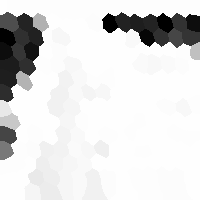
\includegraphics[width=4cm]{experiments/edgebased/normal-vs-inverted/2021-04-18-06:06:02house-l_conv_a0_s0_Dbiased:_Ucycle:_Csuperpixels:20_c10_m0_t50000B_}
                }
                \hspace{8pt}
                \subfloat[][]{
                    \label{fig:exp-edge-pher}
                    
\includegraphics[width=4cm]{experiments/edgebased/normal-vs-inverted/2021-04-18-06:06:02house-l_pher_a0_s0_Dbiased:_Ucycle:_Csuperpixels:20_c10_m0_t50000B_}
                }
                \hspace{8pt}
                \subfloat[][]{
                    \label{fig:exp-edge-steg}
                    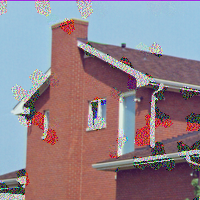
\includegraphics[width=4cm]{experiments/edgebased/normal-vs-inverted/2021-04-18-06:06:02house-l_steg_a0_s0_Dbiased:_Ucycle:_Csuperpixels:20_c10_m0_t50000B_}
                } \\
                \subfloat[][]{
                    \label{fig:exp-edge-inv-conv}
                    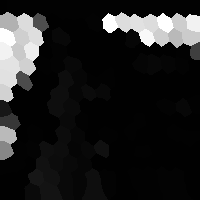
\includegraphics[width=4cm]{experiments/edgebased/normal-vs-inverted/2021-04-18-06:06:25house-l_conv_a0_s0_Dbiased:_Ucycle:_Ci:superpixels:20_c10_m0_t50000B_}
                }
                \hspace{8pt}
                \subfloat[][]{
                    \label{fig:exp-edge-inv-pher}
                    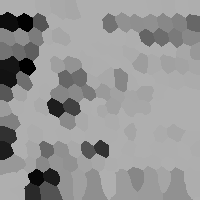
\includegraphics[width=4cm]{experiments/edgebased/normal-vs-inverted/2021-04-18-06:06:25house-l_pher_a0_s0_Dbiased:_Ucycle:_Ci:superpixels:20_c10_m0_t50000B_}
                } \subfloat[][]{
                    \label{fig:exp-edge-inv-steg}
                    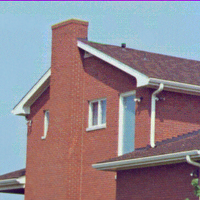
\includegraphics[width=4cm]{experiments/edgebased/normal-vs-inverted/2021-04-18-06:06:25house-l_steg_a0_s0_Dbiased:_Ucycle:_Ci:superpixels:20_c10_m0_t50000B_}
                }

                \caption[Porównania wizualizacji konwersji oraz macierzy maskujących.]
                {Porównania wizualizacji konwersji, macierzy maskujących oraz uzyskanych steganogramów. W pierwszym
                    wierszu (\subref{fig:exp-edge-conv}, \subref{fig:exp-edge-pher}, \subref{fig:exp-edge-steg})
                    przedstawiono obrazy związane z procesem o długości krawędzi odwrotnie proporcjonalnej do różnicy
                    wariancji pikseli należących do segmentów. W drugim wierszu (\subref{fig:exp-edge-inv-conv},
                    \subref{fig:exp-edge-inv-pher}, \subref{fig:exp-edge-inv-steg}) długości są proporcjonalne do
                    różnicy wariancji. Pierwsza kolumna przedstawia wizualizacje procesu konwersji bitmapy na graf,
                    druga przestawia uzyskane macierze maskujące, trzecia zawiera uzyskane steganogramy zawierające
                    $50kB$ informacji}
                \label{fig:exp-edge}
            \end{figure}

            \begin{figure}
                \center
                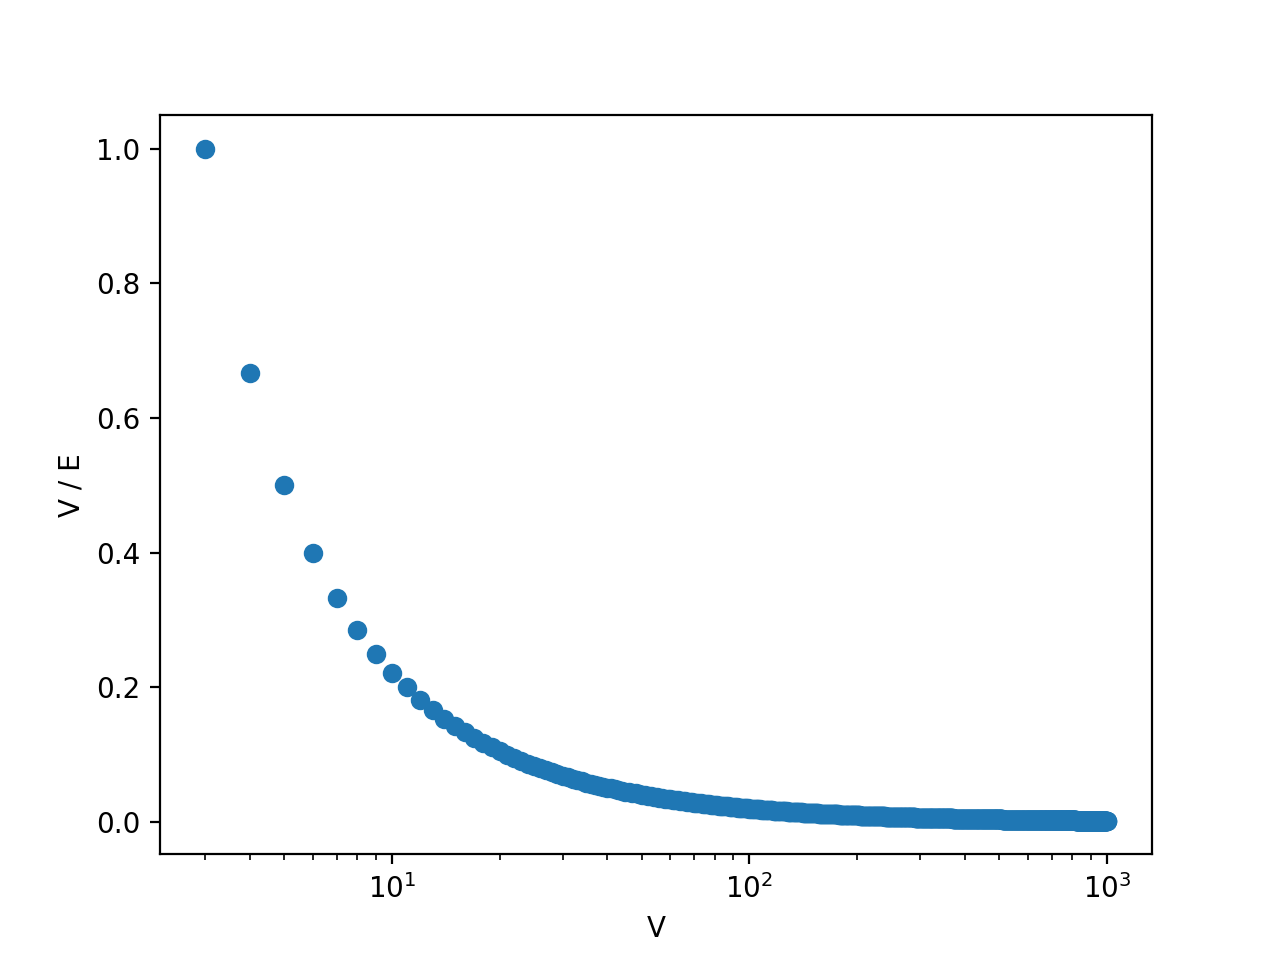
\includegraphics[width=8cm]{experiments/edgebased/normal-vs-inverted/V_vs_E.png}
                \caption
                {Wykres przedstawia stosunek liczby krawędzi należących do cyklu Hamiltona grafu pełnego o $V$
                    wierzchołkach i $E$ krawędziach w zależności od liczby wierzchołków}
                \label{fig:exp-edge-v-vs-e}
            \end{figure}

            % O PARAMETRACH
            Ponieważ rozwiązywany problem był analogiczny do problemu komiwojażera, w trakcie eksperymentów wykorzystano
            optymalne wartości parametry dla każdego z rodzajów systemu wyznaczone podczas testowania poprawności
            działania systemu mrówkowego. Metodę ich wyznaczenia można znaleźć w rozdziale \ref{chap:implementation}.

            % WYNIKI - METODA-KRAWĘDZI - ILOŚĆ SEGMENTÓW
            Ważnym aspektem metody wykorzystującą segmentację obrazu jest dobór docelowej liczby grup pikseli. Wartość
            zbyt niska może powodować powstanie segmentów łączących obszary jednorodne i złożone, co przełoży się na
            zakodowanie nieoptymalnej liczby bitów w wszystkich pikselach segmentu. Zbyt duża liczba, oprócz większej
            liczby obliczeń, może przełożyć się na stworzenie segmentów zbyt małych, których wariancja nie
            będzie wiernie oddawać złożoności całego obszaru.

            Rysunek \ref{fig:exp-edge-method} przedstawia segmentację każdego z obrazów nośnych na zadane liczby
            segmentów z naniesionym śladem feromonowym. W tabeli \ref{tab:exp-edge-results} zawarto wartości miar
            uzyskanych steganogramów dla zadanej pojemności $25kB$ oraz obrazu nośnego o wymiarach $512 \times 512$.

            Dla każdej z metod podziału obrazu osiągnięto zbliżone rezultaty, lecz warto zwrócić uwagę na fakt, że
            metody podziału na prostokąty oraz superpiksele wymagają przekroczenia pewnej wartości granicznej, powyżej
            której osiągane są dobre wyniki. W związku z porównywalnymi wynikami poszczególnych metod podziału obrazu,
            dalej zdecydowano się korzystać z podziału na $20$ superpikseli.

            \begin{figure}
                \centering
                \subfloat[][$N_s = 10$]{
                    \label{fig:exp-edge-method-window1}
                    
\includegraphics[width=4cm]{experiments/edgebased/methods/2021-04-18-09:54:42airplane_pher_scaled_a0_s0_Dbiased:_Ucycle:_Ci:window:10_c10_m0_t250000B_}
                }
                \hspace{8pt}
                \subfloat[][$N_s = 20$]{
                    \label{fig:exp-edge-method-window2}
                    \includegraphics[width=4cm]{experiments/edgebased/methods/2021-04-18-09:54:42airplane_pher_scaled_a0_s0_Dbiased:_Ucycle:_Ci:window:20_c10_m0_t250000B_}
                }
                \hspace{8pt}
                \subfloat[][$N_s = 35$]{
                    \label{fig:exp-edge-method-window3}
                    \includegraphics[width=4cm]{experiments/edgebased/methods/2021-04-18-09:54:43airplane_pher_scaled_a0_s0_Dbiased:_Ucycle:_Ci:window:35_c10_m0_t250000B_}
                } \\
                \subfloat[][$N_s = 10$]{
                    \label{fig:exp-edge-method-superpixel1}
                    \includegraphics[width=4cm]{experiments/edgebased/methods/2021-04-18-09:54:44airplane_pher_scaled_a0_s0_Dbiased:_Ucycle:_Ci:superpixels:10_c10_m0_t250000B_}
                }
                \hspace{8pt}
                \subfloat[][$N_s = 20$]{
                    \label{fig:exp-edge-method-superpixel2}
                    \includegraphics[width=4cm]{experiments/edgebased/methods/2021-04-18-09:54:46airplane_pher_scaled_a0_s0_Dbiased:_Ucycle:_Ci:superpixels:20_c10_m0_t250000B_}
                } \subfloat[][$N_s = 35$]{
                    \label{fig:exp-edge-method-superpixel3}
                    \includegraphics[width=4cm]{experiments/edgebased/methods/2021-04-18-09:54:47airplane_pher_scaled_a0_s0_Dbiased:_Ucycle:_Ci:superpixels:35_c10_m0_t250000B_}
                } \\
                \subfloat[][$N_s = 5$]{
                    \label{fig:exp-edge-method-kmeans1}
                    \includegraphics[width=4cm]{experiments/edgebased/methods/2021-04-18-09:59:31airplane_pher_scaled_a0_s0_Dbiased:_Ucycle:_Ci:kmeans:5_c10_m0_t250000B_}
                }
                \hspace{8pt}
                \subfloat[][$N_s = 10$]{
                    \label{fig:exp-edge-method-kmeans2}
                    \includegraphics[width=4cm]{experiments/edgebased/methods/2021-04-18-09:55:06airplane_pher_scaled_a0_s0_Dbiased:_Ucycle:_Ci:kmeans:10_c10_m0_t250000B_}
                } \subfloat[][$N_s = 20$]{
                    \label{fig:exp-edge-method-kmeans3}
                    \includegraphics[width=4cm]{experiments/edgebased/methods/2021-04-18-09:55:41airplane_pher_scaled_a0_s0_Dbiased:_Ucycle:_Ci:kmeans:20_c10_m0_t250000B_}
                }

                \caption[Macierze maskujące.]
                {Macierze maskujące uzyskane przy podziale obrazu na nienachodzące prostokąty
                    (\subref{fig:exp-edge-method-window1}, \subref{fig:exp-edge-method-window2},
                    \subref{fig:exp-edge-method-window3}), superpiksele (\subref{fig:exp-edge-method-superpixel1},
                    \subref{fig:exp-edge-method-superpixel2}, \subref{fig:exp-edge-method-superpixel3}) i zbiory
                    wyznaczone metodą \textit{k}-średnich (\subref{fig:exp-edge-method-kmeans1},
                    \subref{fig:exp-edge-method-kmeans2}, \subref{fig:exp-edge-method-kmeans3})
                }
                \label{fig:exp-edge-method}
            \end{figure}

            \begin{table}
                \centering
                \caption{Miary jakości w zależności od metody segmentacji obrazu. W tabeli pogrubiono wartości poszczególnych miar wskazujące na najniższy spadek jakości}
                \begin{tabular}{ |l|c|c c c| }
                    \hline
                    Metoda segmentacji & liczba segmentów & $MSE$ & $PSNR$ & $SSIM$ \\
                    \hline
                    Podział na prostokąty & 10   ($V=5$)  & 1764.78 & 15.6978dB & 0.186649 \\
                                        & 21   ($V=7$)  & 1764.78 & 15.6978dB & 0.186649 \\
                                        & 45   ($V=10$) & 27.2669 & 33.8084dB & 0.891967 \\
                                        & 190  ($V=20$) & 7.25700 & 39.5572dB & \textbf{0.948116} \\
                                        & 595  ($V=35$) & 6.85841 & 39.8025dB & 0.947396 \\
                                        & 1225 ($V=50$) & \textbf{6.85694} & \textbf{39.8034dB} & 0.947764 \\
                    \hline
                    Superpiksele          & 10   ($V=5$)  & 1764.78 & 15.6978dB & 0.186649 \\
                                        & 21   ($V=7$)  & 21.7769 & 34.7848dB & 0.903446 \\
                                        & 45   ($V=10$) & 19.2949 & 35.3103dB & 0.913704 \\
                                        & 190  ($V=20$) & 7.07101 & 39.6699dB & \textbf{0.948129} \\
                                        & 595  ($V=35$) & 6.90553 & 39.7728dB & 0.946333 \\
                                        & 1225 ($V=50$) & \textbf{6.77511} & \textbf{39.8556dB} & 0.945946 \\
                    \hline
                    Grupowanie \textit{k}-średnich & 10   ($V=5$)  & 7.89710 & 39.1901dB & 0.940743 \\
                                        & 21   ($V=7$)  & 7.63390 & 39.3373dB & 0.94536 \\
                                        & 45   ($V=10$) & 7.30898 & 39.5262dB & 0.948244 \\
                                        & 190  ($V=20$) & 6.90061 & 39.7759dB & 0.948481 \\
                                        & 595  ($V=35$) & \textbf{6.76695} & \textbf{39.8608dB} & \textbf{0.949062} \\
                                        & 1225 ($V=50$) & - & - & - \\
                    \hline
                \end{tabular}
                \label{tab:exp-edge-results}
            \end{table}

            % METODA KRAWĘDZI - FINAL SHOWDOWN
            Ostatnim krokiem badań metody opartej na wierzchołkach, było porównanie uzyskanych wyników na pozostałych
            obrazach testowych. Uzyskane rezultaty zawiera tabela \ref{tab:exp-edge-results}, a steganogramy przedstawia
            rysunek \ref{fig:exp-edge-results}.

            \begin{table}
                \centering
                \caption{Wyniki uzyskane metodą opartą na wierzchołkach}
                \begin{tabular}{ |l|c|c c c| }
                    \hline
                    Obraz & objętość danych & $MSE$ & $PSNR$ & $SSIM$ \\
                    \hline
                    Baboon {\footnotesize $512 \times 512$}   & 100 000B (12.71\%) & 0.893791 & 48.6524dB & 0.99839 \\
                    Baboon {\footnotesize $512 \times 512$}   & 250 000B (31.78\%) & 7.52079 & 39.4021dB & 0.987705 \\
                    Baboon {\footnotesize $512 \times 512$}   & 500 000B (63.57\%) & 663.829 & 19.9442dB & 0.723623 \\
                    Airplane {\footnotesize $512 \times 512$} & 100 000B (12.71\%) & 0.589252 & 50.4617dB & 0.995266 \\
                    Airplane {\footnotesize $512 \times 512$} & 250 000B (31.78\%) & 7.07101 & 39.6699dB & 0.948129 \\
                    Airplane {\footnotesize $512 \times 512$} & 500 000B (63.57\%) & 362.857 & 22.5674dB & 0.510537 \\
                    Peppers {\footnotesize $512 \times 512$}  & 100 000B (12.71\%) & 0.586621 & 50.4812dB & 0.995526 \\
                    Peppers {\footnotesize $512 \times 512$}  & 250 000B (31.78\%) & 7.21685 & 39.5813dB & 0.951955 \\
                    Peppers {\footnotesize $512 \times 512$}  & 500 000B (63.57\%) & 411.621 & 22.0198dB & 0.47874 \\
                    \hline
                \end{tabular}
                \label{tab:exp-edge-results}
            \end{table}

            \begin{figure}
                \footnotesize
                \centering
                \subfloat[][$D = 100 000B$]{
                    \label{fig:exp-edge-results-baboon-100k}
                    \includegraphics[width=3cm]{experiments/edgebased/results/2021-04-18-12:17:54mandrill_steg_a0_s0_Dbiased:_Ucycle:_Ci:superpixels:20_c10_m0_t100000B_}
                }
                \hspace{8pt}
                \subfloat[][$D = 250 000B$]{
                    \label{fig:exp-edge-results-baboon-250k}
                    \includegraphics[width=3cm]{experiments/edgebased/results/2021-04-18-12:17:54mandrill_steg_a0_s0_Dbiased:_Ucycle:_Ci:superpixels:20_c10_m0_t250000B_}
                }
                \hspace{8pt}
                \subfloat[][$D = 500 000B$]{
                    \label{fig:exp-edge-results-baboon-500k}
                    \includegraphics[width=3cm]{experiments/edgebased/results/2021-04-18-12:17:54mandrill_steg_a0_s0_Dbiased:_Ucycle:_Ci:superpixels:20_c10_m0_t500000B_}
                } \\
                \subfloat[][$D = 100 000B$]{
                    \label{fig:exp-edge-results-aiplane-100k}
                    \includegraphics[width=3cm]{experiments/edgebased/results/2021-04-18-12:17:54airplane_steg_a0_s0_Dbiased:_Ucycle:_Ci:superpixels:20_c10_m0_t100000B_}
                }
                \hspace{8pt}
                \subfloat[][$D = 250 000B$]{
                    \label{fig:exp-edge-results-aiplane-250k}
                    \includegraphics[width=3cm]{experiments/edgebased/results/2021-04-18-12:17:54airplane_steg_a0_s0_Dbiased:_Ucycle:_Ci:superpixels:20_c10_m0_t250000B_}
                }
                \hspace{8pt}
                \subfloat[][$D = 500 000B$]{
                    \label{fig:exp-edge-results-aiplane-500k}
                    \includegraphics[width=3cm]{experiments/edgebased/results/2021-04-18-12:17:54airplane_steg_a0_s0_Dbiased:_Ucycle:_Ci:superpixels:20_c10_m0_t500000B_}
                } \\
                \subfloat[][$D = 100 000B$]{
                    \label{fig:exp-edge-results-airplane-100k}
                    \includegraphics[width=3cm]{experiments/edgebased/results/2021-04-18-12:17:54peppers_steg_a0_s0_Dbiased:_Ucycle:_Ci:superpixels:20_c10_m0_t100000B_}
                }
                \hspace{8pt}
                \subfloat[][$D = 250 000B$]{
                    \label{fig:exp-edge-results-airplane-250k}
                    \includegraphics[width=3cm]{experiments/edgebased/results/2021-04-18-12:17:54peppers_steg_a0_s0_Dbiased:_Ucycle:_Ci:superpixels:20_c10_m0_t250000B_}
                }
                \hspace{8pt}
                \subfloat[][$D = 500 000B$]{
                    \label{fig:exp-edge-results-airplane-500k}
                    \includegraphics[width=3cm]{experiments/edgebased/results/2021-04-18-12:17:54peppers_steg_a0_s0_Dbiased:_Ucycle:_Ci:superpixels:20_c10_m0_t500000B_}
                }

                \caption[Porównanie rezultatów]
                {Porównanie uzyskanych steganogramów przy zadanej objętości ukrytej informacji}
                \label{fig:exp-edge-results}
            \end{figure}
        }
    }

    % OCENA SUBIEKTYWNA
    \section{Ocena subiektywna}
    {
        Uzyskane steganogramy spełniają postawione przed nimi oczekiwania. Dla obrazów w których wykorzystano $\sim
        32\%$ dostępnej objętości zmiany są praktycznie niezauważalne gołym okiem. Artefakty stały się dopiero wyraźnie
        widoczne gdy spróbowano ukryć $500kB$, czyli blisko $64\%$ objętości. W przypadku metody opartej na podziale
        obrazu na grupy pikseli, były one bardziej widoczne, gdyż występowały krawędzie pomiędzy superpikselami lub
        prostokątami dzielącymi obraz. Metoda budowania grafu na podstawie wierzchołków gwarantowała płynniejsze
        przejścia pomiędzy obszarami, w których wykorzystano większą liczbę bitów pikseli.

        Warto również podkreślić zgodność subiektywnych odczuć z wartościami przedstawionych miar jakości. Dodatkowo,
        przytoczony zakres szczytowego stosunku sygnału do szumu, $30dB - 50dB$, pokrywa się z doznaniami empirycznymi.
        Dla akceptowalnych steganogramów wykorzystujących $\sim 32\%$ pojemności, wartość $PSNR$ wynosiła blisko $40dB$.
        W przypadku wykorzystania $\sim 64\%$ bitów obrazu, wartość $PSNR$ spadła do nieakceptowalnego poziomu bliskiemu
        $20dB$.

        Kolejna interesująca obserwacja płynie z porównania efektów ukrywania informacji w obrazie \textit{Baboon} i
        \textit{Airplane}. Nawet w przypadku ukrycia blisko $500kB$ danych, były one ewidentnie bardziej widoczne w
        obrazie \textit{Airplane}. Może to być tłumaczone dużo większym zróżnicowaniem obrazu \textit{Baboon}, oraz
        większą liczbą szczegółów i tekstur.
    }

    % PORÓWNANIE Z INNYMI METODAMI
    \section{Porównanie wyników z innymi metodami}
    {
        Ostatnim krokiem związanym z badaniem efektywności zaproponowanych metod było porównanie uzyskanych wyników do
        powiązanych prac z dziedziny. Udostępnione wyniki badań pozwoliły na utworzenie porównującego zestawienia z
        metodą \textit{Least Significant Bit} \cite{Solak2018LSBSA}, \textit{Pixel Value
        Differencing} \cite{Solak2018LSBSA}, \textit{Particle Swarm Optimization-Integer Wavelet
        Transform} \cite{Muhuri2020ANI} oraz metodą opartą na wykrywaniu złożonego regionu obrazu za pomocą systemu
        mrowiskowego \cite{Khan2018AntCO}, do której odniesienie można znaleźć w rozdziale \ref{chap:stegoants}.

        W związku z tym, że w powyższych artykułach przedstawione wyniki zostały podane dla różnych objętości ukrywanych
        informacji, zdecydowano się umieścić poszczególne porównania w osobnych tabelach. Format zapisu wyników był
        niejednolity, część prac wyrażała uzyskaną pojemność w postaci udziału procentowego bitów obrazu nośnego, liczby
        bitów w przeliczeniu na piksel (\textit{bpp}) lub bezwzględnej liczby bajtów. Ponieważ obrazy, na których
        wykonywano eksperymenty są znane, możliwe było ustandaryzowanie przytoczonych wartości.

        Zestawienia z poszczególnymi pracami zawierają tabele \ref{tab:exp-comparison-lsb},
        \ref{tab:exp-comparison-pvd}, \ref{tab:exp-comparison-pso-iwt} oraz \ref{tab:exp-comparison-aco}. W kolumnach
        zawierających wartości miar pogrubiono wartości wskazujące na najniższą degradację obrazu.

        % pod każdą tabelą pojawiła się krótka interpretacja jej zawartości (z konkretami)

        \begin{table}[H]
            \footnotesize
            \centering
            \caption{Porównanie miar jakości z uzyskanymi metodą \textit{LSB} w pracy \cite{Solak2018LSBSA}}
            \resizebox{\textwidth}{!}
            {
            \begin{tabular}{ |l|c c c|c c c|c c c|c c c| }
                \hline
                & \multicolumn{3}{c|}{pojemność}
                & \multicolumn{3}{c|}{\textit{Least Significant Bit}}
                & \multicolumn{3}{p{4.5cm}|}{\centering Metoda oparta na \\ wierzchołkach}
                & \multicolumn{3}{p{4.5cm}|}{\centering Metoda oparta na \\ krawędziach} \\
                \hline
                Obraz & $bpp$ & $\%$ & $B$ & {\scriptsize $MSE$} & {\scriptsize $PSNR$} & {\scriptsize $SSIM$} & {\scriptsize $MSE$} & {\scriptsize $PSNR$} & {\scriptsize $SSIM$} & {\scriptsize $MSE$} & {\scriptsize $PSNR$} & {\scriptsize $SSIM$} \\
                \hline
                \hline
                Airplane & 2.67 & 11.12\% & 87491B
                    & -     & 51.65dB & \textbf{0.9970}
                    & 0.447 & \textbf{51.66dB} & 0.9963
                    & 0.448 & 51.65dB & 0.9963 \\

                Baboon & 2.67 & 11.12\% & 87491B
                    & -     & \textbf{51.65dB} & \textbf{0.9997}
                    & 0.449 & 51.64dB & 0.9990
                    & 0.816 & 49.05dB & 0.9985 \\

                Peppers & 2.67 & 11.12\% & 87491B
                    & -     & 51.62dB & \textbf{0.9998}
                    & 0.448 & 51.65dB & 0.9968
                    & 0.447 & \textbf{51.66dB} & 0.9967 \\
                \hline
            \end{tabular}
            }
            \label{tab:exp-comparison-lsb}
        \end{table}

        Na podstawie tabeli \ref{tab:exp-comparison-lsb}, porównującej wyniki uzyskane techniką \textit{LSB} oraz
        metodami zaproponowanymi w niniejszej pracy, trudno rozstrzygnąć wyższość jednego podejścia nad drugim. Dla
        każdego z testowych obrazów, wartości miary \textit{SSIM} były korzystniejsze dla steganogramów uzyskanych
        metodą \textit{LSB}. Wartości szczytowego stosunku sygnału do szumu (\textit{PSNR}) były zbliżone dla wszystkich
        podejść.

        Taki wynik można próbować tłumaczyć charakterystyką miary \textit{SSIM}, która kładzie znaczący nacisk na zmiany
        struktury obrazu. Metoda \textit{LSB} z punktu widzenia obrazu wprowadza jednorodny szum na stałym poziomie, co
        w małym stopniu wpływa na jego strukturę i w rezultacie powoduje mniejszy spadek wartości miary.

        \begin{table}[H]
            \footnotesize
            \centering
            \caption{Porównanie miar jakości z uzyskanymi metodą \textit{PVD} w pracy \cite{Solak2018LSBSA}}
            \resizebox{\textwidth}{!}
            {
            \begin{tabular}{ |l|c c c|c c c|c c c|c c c| }
                \hline
                & \multicolumn{3}{c|}{pojemność}
                & \multicolumn{3}{c|}{\textit{Pixel Value Differencing}}
                & \multicolumn{3}{p{4.5cm}|}{\centering Metoda oparta na \\ wierzchołkach}
                & \multicolumn{3}{p{4.5cm}|}{\centering Metoda oparta na \\ krawędziach} \\
                \hline
                Obraz & $bpp$ & $\%$ & $B$ & {\scriptsize $MSE$} & {\scriptsize $PSNR$} & {\scriptsize $SSIM$} & {\scriptsize $MSE$} & {\scriptsize $PSNR$} & {\scriptsize $SSIM$} & {\scriptsize $MSE$} & {\scriptsize $PSNR$} & {\scriptsize $SSIM$} \\
                \hline
                \hline
                Airplane & 4.6699 & 19.45\% & 153023B
                    & -     & 40.61dB & 0.9751
                    & 1.596 & \textbf{46.13dB} & \textbf{0.9879}
                    & 1.645 & 46.00dB & 0.9865 \\
                Baboon & 5.3627 & 22.34\% & 175725B
                    & -     & 37.83dB & 0.9945
                    & 2.012 & \textbf{45.13dB} & \textbf{0.9960}
                    & 2.647 & 43.94dB & 0.9953 \\
                Peppers & 4.7177 & 19.65\% & 154590B
                    & -     & 40.93dB & \textbf{0.9980}
                    & 1.638 & \textbf{46.21dB} & 0.9892
                    & 1.684 & 45.90dB & 0.9878 \\
                \hline
            \end{tabular}
            }
            \label{tab:exp-comparison-pvd}
        \end{table}

        Porównanie opracowanych metod z wynikami uzyskanymi metodą \textit{PVD} (tabela \ref{tab:exp-comparison-pvd})
        wypada na zdecydowaną korzyść metody opartej na budowie grafu poczynając od wierzchołków. Uzyskane wartości
        \textit{PSNR} znacząco przewyższały rezultaty przedstawione w pracy \cite{Solak2018LSBSA}. Wartości
        \textit{SSIM} były bardzo zbliżone, lecz w dwóch z trzech obrazów były one korzystniejsze dla zaproponowanej
        metody.

        \begin{table}[H]
            \footnotesize
            \centering
            \caption{Porównanie miar jakości z uzyskanymi metodą \textit{PSO-IWT} w pracy \cite{Muhuri2020ANI}}
            \resizebox{\textwidth}{!}
            {
            \begin{tabular}{ |l|c|c c c|c c c|c c c| }
                \hline
                & \multicolumn{1}{c|}{pojemność}
                & \multicolumn{3}{c|}{\textit{PSO-IWT}}
                & \multicolumn{3}{p{4.5cm}|}{\centering Metoda oparta na \\ wierzchołkach}
                & \multicolumn{3}{p{4.5cm}|}{\centering Metoda oparta na \\ krawędziach} \\
                \hline
                Obraz & $B$ & {\scriptsize $MSE$} & {\scriptsize $PSNR$} & {\scriptsize $SSIM$} & {\scriptsize $MSE$} & {\scriptsize $PSNR$} & {\scriptsize $SSIM$} & {\scriptsize $MSE$} & {\scriptsize $PSNR$} & {\scriptsize $SSIM$} \\
                \hline
                \hline
                Airplane & 73728B
                    & -     & 41.13dB & -
                    & 0.378 & \textbf{52.39dB} & 0.9971
                    & 0.378 & 52.39dB & 0.9968 \\
                Baboon & 73728B
                    & -     & 41.38dB& -
                    & 0.379 & \textbf{52.38dB} & 0.9993
                    & 0.378 & 52.38dB & 0.9993 \\
                \hline
            \end{tabular}
            }
            \label{tab:exp-comparison-pso-iwt}
        \end{table}

        Wyniki zestawienia z metodą \textit{PSO-IWT} opisaną w pracy \cite{Muhuri2020ANI} również wypadają pozytywnie
        (tabela \ref{tab:exp-comparison-pso-iwt}). Z powodu braku referencyjnych wartości miary \textit{SSIM}, możliwe
        jest jedynie odniesienie się do miary \textit{PSNR}, której wartości są wyższe o blisko rząd wielkości.

        \begin{table}[H]
            \footnotesize
            \centering
            \caption{Porównanie miar jakości z uzyskanymi metodą \textit{ACO} w pracy \cite{Khan2018AntCO}}
            \resizebox{\textwidth}{!}
            {
            \begin{tabular}{ |l|c c|c c c|c c c|c c c| }
                \hline
                & \multicolumn{2}{c|}{pojemność}
                & \multicolumn{3}{c|}{\textit{PSO-IWT}}
                & \multicolumn{3}{p{4.5cm}|}{\centering Metoda oparta na \\ wierzchołkach}
                & \multicolumn{3}{p{4.5cm}|}{\centering Metoda oparta na \\ krawędziach} \\
                \hline
                Obraz & \% & $B$ & {\scriptsize $MSE$} & {\scriptsize $PSNR$} & {\scriptsize $SSIM$} & {\scriptsize $MSE$} & {\scriptsize $PSNR$} & {\scriptsize $SSIM$} & {\scriptsize $MSE$} & {\scriptsize $PSNR$} & {\scriptsize $SSIM$} \\
                \hline
                \hline
                Baboon & 2.8473\% & 22396B
                    & 0.8409 & 48.88dB & -
                    & 0.1151 & 57.55dB & 0.9999
                    & \textbf{0.1146} & \textbf{57.57dB} & 0.9998 \\
                Pepper & 2.8661\% & 22544B
                    & 1.0605 & 47.88dB & -
                    & 0.1151 & \textbf{57.56dB} & 0.9994
                    & \textbf{0.1150} & \textbf{57.56dB} & 0.9991 \\
                \hline
            \end{tabular}
            }
            \label{tab:exp-comparison-aco}
        \end{table}

        Podobnie do poprzednich zestawień, tabela \ref{tab:exp-comparison-aco} ukazuje porównanie wyników uzyskanych
        opracowanymi metodami oraz metodą im najbliższą, gdyż również wykorzystującą system mrówkowy do wyszczególnienia
        złożonych obszarów obrazu. Wartości miar \textit{PSNR} oraz \textit{SSIM} wskazują na wyższość zaproponowanej
        metody w aspekcie stosunku utraty jakości do pojemności steganogramu. W przeciwieństwie do poprzednich
        zestawień, minimalnie lepsze rezultaty uzyskano metodą opartą na krawędziach.
        %
    }

    \section{Podsumowanie wyników eksperymentów}
    {
        % omówienie wyników wszystkich eksperymentów, bez konkretnych liczb, ale za to ich interpretacja i dyskusja
        Przeprowadzone eksperymenty pozwalają na wyciągnięcie wielu interesujących wniosków. Po pierwsze, obydwie
        zaproponowane metody - budująca graf poczynając od wierzchołków lub od krawędzi - są poprawne, i pozwalają na
        sterowanie procesem ukrywania danych w obrazach. Głównym kryterium, które posłużyło do oceny metod był ich wpływ
        na degradację obrazu w zależności od objętości ukrywanych danych. Na jego podstawie, po odpowiednim dobraniu
        parametrów procesu, możliwe jest osiągnięcie wyników zbliżonych, lub nawet lepszych względem prac opisujących
        obecny stan techniki \cite{Solak2018LSBSA, Muhuri2020ANI, Khan2018AntCO}.

        Obydwie zaproponowane w niniejszej pracy metody łączą założenia oraz ogólny mechanizm działania. Ich różnice,
        związane z metodą konstrukcji grafu na podstawie bitmapy są ewidentne, lecz mimo tego, uzyskiwane za ich pomocą
        rezultaty były zbliżone pod kątem przytoczonych miar jakości w podrozdziale \ref{sec:measures}. Fakt ten, można
        interpretować jako pozytywną weryfikację założeń, m.in. o słuszności wykorzystania złożonych obszarów obrazów,
        szczegółowo opisanych w rozdziale \ref{sec:assumptions}.

        Parametrem, posiadającym najbardziej znaczący wpływ na uzyskiwane rezultaty, była relacja długości krawędzi
        grafu do różnic między pikselami lub ich grupami. Badania wykazały znaczącą wyższość podejścia w którym
        odległości są proporcjonalne do różnic pikseli lub wariancji wewnątrz ich grupy. Realizacja takiego podejścia
        powoduje intensywniejsze odkładanie się śladu feromonowego w mało zróżnicowanych obszarach obrazu i wymusza
        stosowanie odwrotności macierzy maskującej podczas etapu ukrywania danych. Można doszukiwać się wielu przyczyn
        takiego stanu rzeczy. Przykładowo, jednym z jego powodów może być względna mniejsza ilość złożonych obszarów
        obrazów do obszarów o niskiej złożoności. Alternatywnie, obszary złożone obrazów mogą być częściej oddzielone od
        siebie obszarami mniej złożonymi. Obydwa przypadki utrudniają mrówkom swobodne poruszanie się bo całej
        przestrzeni obrazu, co prowadzi do zbyt skupionego odkładania się śladu, czego przykładem może być rysunek
        \ref{fig:exp-edge-steg}.

        Interesującym elementem rozróżniającym obydwie zaproponowane metody, jest charakter problemu reprezentowany
        przez graf. W przypadku metody opartej na budowie grafu poczynając od wierzchołków, problem stawiony przed
        wirtualnymi mrówkami nie był analogiczny do problemu komiwojażera, i wymagał pewnych adaptacji opisanych w
        podrozdziale \ref{subsec:vertex-method}. Znacząco utrudniło to przeprowadzanie badań i ocenę algorytmu, ponieważ
        heurystyki doboru parametrów systemów mrówkowych okazywały się nieskuteczne. Ponadto, powyższa metoda jest
        bardzo czuła na wybrany rodzaj systemu mrówkowego, i okazała się zupełnie nieskuteczna dla systemu mrowiskowego
        i systemu max-min \ref{fig:exp-vertex-pher}. Taki stan rzeczy można próbować tłumaczyć ich silną faworyzacją
        jedynie najkrótszej znalezionej ścieżki, co okazuje się nie odpowiadać charakterowi tego zadania. Metody oparte
        na konstrukcji grafu poczynając od krawędzi były pozbawione powyższych wad. Reprezentowany problem był
        analogiczny do problemu komiwojażera, przez co możliwe było wykorzystanie wskazówek oraz wyznaczonych
        doświadczalnie heurystyk doboru parametrów systemu.

        Ponieważ obydwie metody gwarantują zbliżone rezultaty, możliwe jest wybranie metody o niższym zapotrzebowaniu na
        zasoby procesora. Podczas przeprowadzanych eksperymentów, najmniej obciążające były metody oparte na podziale
        obrazu na superpiksele oraz nienachodzące prostokąty. Z względu na regularne krawędzie oddzielające grupy
        pikseli w których ukryto te same liczby bitów, które występują przy segmentacji na prostokąty, wskazane jest
        korzystanie z segmentacji na superpiksele.
        %
    }
    %
}

% BADANIE PERCEPCJI I OCENY OBRAZÓW
% file:///Users/grzegorzkazana/Desktop/Stegano_Ant/Comparisonoffoursubjectivemethodsforimagequalityassessment.pdf
% file:///Users/grzegorzkazana/Desktop/Stegano_Ant/ImageQualityAssessment.pdf
% file:///Users/grzegorzkazana/Desktop/Stegano_Ant/Contrast_masking_in_human_vision.pdf

% SSIM https://www.cns.nyu.edu/pub/eero/wang03-reprint.pdf
% SSIM vs PSNR https://www.semanticscholar.org/paper/Image-Quality-Metrics%3A-PSNR-vs.-SSIM-Hor%C3%A9-Ziou/4a9a98cc86b1e07e548b7edee045275a793f6698

% WYNIKI INNYCH PRAC
% - lsb/dvt
% https://www.researchgate.net/publication/329245499_LSB_Substitution_and_PVD_performance_analysis_for_image_steganography
%
% - jakaś nakoksana metoda
% file:///Users/grzegorzkazana/Desktop/Stegano_Ant/A%20novel%20algorithm%20for%20colour%20image%20steganography%20using%20a%20new%20intelligent%20technique%20based%20on%20three%20phases.pdf
%
% - wariacje IWT + sztosowe porównanie str. 24
%   file:///Users/grzegorzkazana/Desktop/Stegano_Ant/A%20Novel%20Image%20Steganographic%20Method%20based%20on%20Integer%20Wavelet%20Transformation%20and%20Particle%20Swarm%20Optimization.pdf
%
% - ACO steganography str. 6
%   file:///Users/grzegorzkazana/Desktop/Stegano_Ant/Ant%20Colony%20Optimization%20ACO%20based%20Data%20Hiding%20in%20Image%20Complex%20Region.pdf
%
% - vivbs
% file:///Users/grzegorzkazana/Desktop/Stegano_Ant/Varying_index_varying_bits_substitution_algorithm_.pdf

% find docs/thesis/assets/images/experiments/**/*.bmp | ggrep  -oP '^[\w/_:\.,-]+(?=\.bmp)'  | xargs -I XXX convert XXX.bmp XXX.png